\documentclass[a4paper, 12pt]{article}
\usepackage[a4paper]{geometry}
\usepackage[myheadings]{fullpage}
\usepackage{fancyhdr}
\usepackage{lastpage}
\usepackage{graphicx, wrapfig, subcaption, setspace, booktabs}
\usepackage[T1]{fontenc}
\usepackage[font=small, labelfont=bf]{caption}
\usepackage{fourier}
\usepackage[protrusion=true, expansion=true]{microtype}
\usepackage[english,slovene]{babel}
\usepackage{sectsty}
\usepackage{url, lipsum}
\usepackage{amsmath}
%Če maš slike v mapi slike v tem direktoriju
\graphicspath{{./slike/}}

%math quotation
\newsavebox{\mathbox}\newsavebox{\mathquote}
\makeatletter
\newcommand{\mathquotes}[1]{% \mathquotes{<stuff>}
  \savebox{\mathquote}{\text{``}}% Save quotes
  \savebox{\mathbox}{$\displaystyle #1$}% Save <stuff>
  \raisebox{\dimexpr\ht\mathbox-\ht\mathquote\relax}{``}#1\raisebox{\dimexpr\ht\mathbox-\ht\mathquote\relax}{''}
}
\makeatother


% Neki za obliko (glava, noga)
\newcommand{\HRule}[1]{\rule{\linewidth}{#1}}
\doublespacing
\setcounter{tocdepth}{5}
\setcounter{secnumdepth}{5}

%-------------------------------------------------------------------------------
% DEFINICIJE, IZREKI, DOKAZI
%-------------------------------------------------------------------------------
% Da ni pike na koncu definicije (namesto Definicija 1. bo pisalo Definicija 1)
\usepackage{amsthm}
\usepackage{xpatch}
\makeatletter
\AtBeginDocument{\xpatchcmd{\@thm}{\thm@headpunct{.}}{\thm@headpunct{}}{}{}}
\makeatother

%Definicije, izreki, trditve ...
\newtheorem{lema}{Lema}[section]
\newtheorem*{zgled}{Zgled: }
\newtheorem{trditev}[lema]{Trditev}
\newtheorem{izrek}[lema]{Izrek}
\newtheorem{definicija}{Definicija}[section]
\theoremstyle{definition}
\newtheorem{primer}{Primer}[section]
\newtheorem{posledica}[lema]{Posledica}
\newtheorem*{opomba}{Opomba:}

% \newenvironment{theo}
%    {\begin{shaded}\begin{theorem}}
%    {\end{theorem}\end{shaded}}

%-------------------------------------------------------------------------------
% HEADER & FOOTER
%-------------------------------------------------------------------------------

% oblika (naslovnica, glava, noga)
\pagestyle{fancy}
\fancyhf{}
\setlength\headheight{15pt}
\fancyhead[L]{Aljaž Ostrež, Renyi divergenca}
\fancyhead[R]{Ljubljana, \today}
\fancyfoot[R]{Stran \thepage}

\renewcommand{\headrulewidth}{2pt}
\renewcommand{\footrulewidth}{1pt}

% Poljubno
\newcommand{\N}{\mathcal{N}}
\newcommand{\RR}{\mathbb{R}}

%-------------------------------------------------------------------------------
% TITLE PAGE
%-------------------------------------------------------------------------------

\begin{document}

% Oblika naslova
\title{ \HRule{2pt} \\
        \LARGE \textbf{\uppercase{Divergenca kot merilo za razliko med porazdelitvami}}
        \HRule{2pt} \\ [0.5cm]
        \normalsize \vspace*{5\baselineskip}}

\author{
        Aljaž Ostrež \\ 
		Fakulteta za matematiko in fiziko, Ljubljana \\ 
		Institut Jožefa Stefana, Ljubljana \\}

\maketitle
\thispagestyle{empty}
\newpage

\setcounter{page}{1}

%-------------------------------------------------------------------------------
% TABLE OF CONTENT
%-------------------------------------------------------------------------------

\tableofcontents
\newpage

%-------------------------------------------------------------------------------
% BODY
%-------------------------------------------------------------------------------

\section*{Uvod}

Verjetnost in statistika sta veji matematike, ki močno povezujeta teoretično matematiko in praktično uporabo matematike v znanosti.

Zakaj pogostokrat v istem stavku govorimo o verjetnosti in statistiki? Statistika in verjetnost sta zelo povezana pojma, saj v statistični teoriji opišemo naključnost in negotovost s pomočjo teorije verjetnosti.

%% KRATEK PREGLED
Najprej bomo opisali osnovne pojme verjetnosti in statistike, ki jih bomo uporabili v nadaljevanju. V naslednjem poglavju bomo opisali pojem divergence (glede na gostoto verjetnosti). V nadaljevanju bomo opisali nekaj metod za predstavitev vzorca podatkov. Pogledali si bomo, kako računamo Renyi divergenco glede na histogram, nato pa opisali še pojem entropije in vpeljali posplošeno Jensenovo divergenco.

Posebna zahvala gre dr. Miranu Černetu iz Fakultete za matematiko in fiziko v Ljubljani, ki mi je pomagal pri dokazu, da je Renyi divergenca res divergenca. Prav tako pa se zahvaljujem mentorjema na Inštitutu Jožefa Stefana v času študija, dr. Pavletu Boškoskemu in dr. Đaniju Juričiću.

\section{Osnovni statistični pojmi}

Na kratko predstavimo statistične pojme, ki jih moramo razumeti za nadaljna poglavja. Definicije niso formalne, saj je namen tega poglavja bralcu razumljivo predstaviti te pojme na enostaven in pregleden način. Bralec, ki dobro pozna osnovne pojme statistike in teorije verjetnosti, lahko to poglavje izpusti.

Začnimo z definicijami osnovnih statističnih pojmov:

\begin{definicija}
	\leavevmode
	\begin{enumerate}
		\item \textbf{Statistična populacija} (ali \textbf{populacija}) je množica vseh proučevanih elementov. Potrebna je natančna časovna in krajevna opredelitev.
		\item Dovolj velika podmnožica populacije, tj. podmnožica, na osnovi katere lahko sklepamo lastnosti celotne populacije, imenujemo \textbf{vzorec}.
		\item Posameznemu proučevanemu elementu populacije/vzorca pravimo \textbf{enota}.
		\item \textbf{Spremenljivka} je lastnost enot.
	\end{enumerate}
\end{definicija}

Poglejmo si primer statistične populacije:

\begin{zgled}
	Vzemimo populacijo vseh študentov v 2. letniku matematike na Fakulteti za matematiko in fiziko (krajevna opredelitev) v šolskem letu 2018/2019 (časovna opredelitev). Če so študenti enakomerno razdeljeni v dve skupini za vaje, je vsaka skupina vzorec populacije. Posamezen študent je enota te populacije, kot spremenljivko pa lahko vzamemo na primer višino, težo, spol, povprečje ocen v tekočem študijskem letu itd.
\end{zgled}

\pagebreak

\textbf{Spremenljivka} je nasprotje od \textbf{konstante}; medtem ko ima konstanta le eno vrednost, spremenljivka zavzame različne vrednosti. Kot je že bilo omenjeno, je spremenljivka lastnost enote statistične populacije. Poznamo več delitev spremenljivk, zaradi naših potreb se bomo omejili le na \textbf{delitev spremenljivk glede na tip izražanja vrednosti}:
\begin{enumerate}
	\item \textbf{Opisne (atributivne) spremenljivke} - vrednosti lahko opišemo z besedami (npr. spol, barva oči, ...).
	\item \textbf{Številske (numerične) spremenljivke} - vrednosti izražamo s števili. Številske spremenljivke delimo še na dve veji:
		\begin{itemize}
			\item \textbf{zvezne}: v teoriji lahko zavzamejo katerokoli vrednost na nekem intervalu (npr. teža, pretečen čas, ...),
			\item \textbf{diskretne}: na nekem intervalu lahko zavzamejo le določene vrednosti (npr. število študentov v posameznem letniku).
		\end{itemize}
\end{enumerate}

Poznamo različne tipe statističnih analiz glede na število hkrati analiziranih spremenljivk:
\begin{itemize}
	\item \textbf{univariatna} - analiza ene spremenljivke,
	\item \textbf{bivariatna} - analiza dveh spremenljivk,
	\item \textbf{multivariatna} - analiza več spremenljivk.
\end{itemize}

Omejili se bomo na univariatno analizo. Omenimo še definicijo slučajne spremenljivke:

\begin{definicija}
	\textbf{Slučajna spremenljivka} je količina, ki nastopi kot rezultat poskusa, kjer je možnih več izidov.
\end{definicija}

V statistiki lahko razumemo slučajno spremenljivko kot spremenljivko naključno izbrane enote statističnega vzorca.

Poglejmo si še definicije porazdelitve, verjetnostne funkcije in funkcije gostote verjetnosti, ker na podlagi teh pojmov temeljijo vsa naslednja poglavja.

\begin{definicija}
	Če za neko slučajno spremenljivko poznamo vse možne izide in vemo, kako pogosto jih zavzame, pravimo, da poznamo njeno \textbf{verjetnostno porazdelitev}.	
\end{definicija}

\begin{zgled}
	\leavevmode
	\begin{enumerate}
		\item Porazdelitev diskretne spremenljivke - rezultat meta dveh kock
		\begin{figure}[!ht]
			\centering
			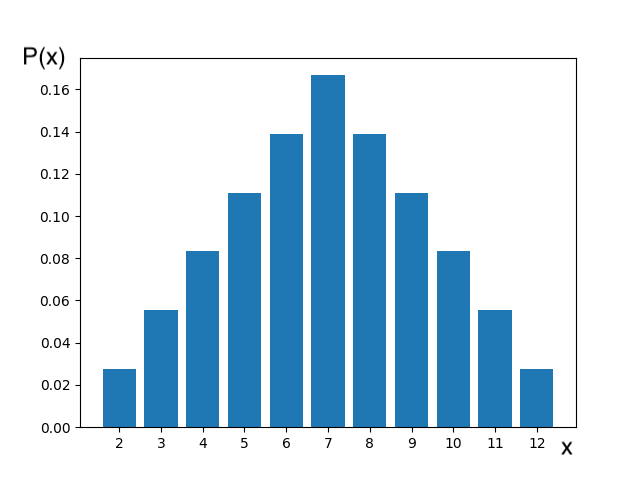
\includegraphics[width=0.5\textwidth]{disk_por}
			\caption{Porazdelitev meta dveh igralnih kock.}
		\end{figure}
		\item Porazdelitev zvezne spremenljivke - inteligenčni količnik (IQ)
		\begin{figure}[!ht]
			\centering
			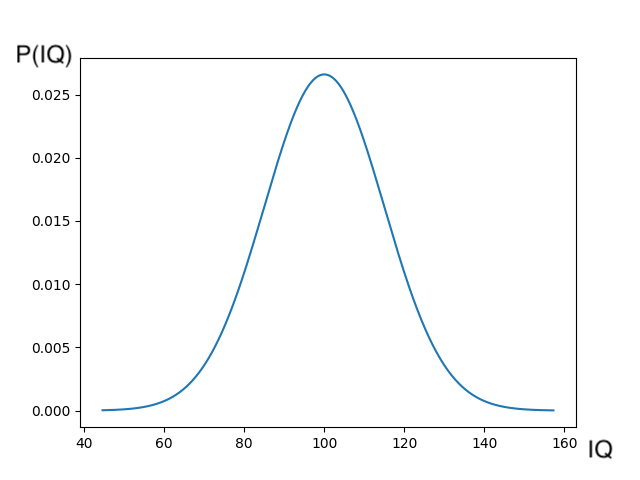
\includegraphics[width=0.5\textwidth]{iq}
			\caption{Porazdelitev IQ v populaciji ljudi.}
		\end{figure}
	\end{enumerate}
\end{zgled}

Vse možne izide porazdelitve in pogostost izidov nam predstavi funkcija verjetnosti za diskretne spremenljivke oziroma funkcija gostote verjetnosti za zvezne spremenljivke. Navedimo natančnejši definiciji:

\begin{definicija}
	\leavevmode
	\begin{itemize}
		\item \textbf{Funkcija gostote verjetnosti} (ali samo gostota verjetnosti, angl. probability density function) zvezne slučajne spremenljivke $X$ je funkcija $f: \mathbb{R} \rightarrow \mathbb{R^+}$, tako da za vsaki realni števili $a \leq b$ velja:
		\begin{equation}
			P(a \leq X \leq b) = \int_a^b f(x) \ dx.
		\end{equation}
		Drugače povedano, ploščina gostote verjetnosti med $a$ in $b$ nam pove, kakšna je verjetnost, da se zgodijo dogodki med $a$ in $b$. Veljati mora še $f(x) \geq 0$ za vse $x$ in $\int_{-\infty}^\infty f(x) \ dx = 1$.
		\item \textbf{Funkcija verjetnosti} (angl. probability mass function) diskretne slučajne spremenljivke $X$ je funkcija $p: \mathbb{R} \rightarrow [0,1]$, definirana kot
		\begin{equation}
			p(a) = P(X = a)
		\end{equation}
		za $a \in \mathbb{R}$, tj. funkcija, ki nam pove, kakšna je verjetnost da se zgodi dogodek $a$ za vse $a$. Veljati mora še $\sum_i p(a_i) = 1$, ko $i$ preteče vse možnosti.
	\end{itemize}
\end{definicija}

S tem, ko poznamo funkcijo verjetnosti oz. gostoto verjetnosti, poznamo tudi porazdelitev slučajne spremenljivke.

Poglejmo si še nekaj porazdelitev zveznih spremenljivk.

\begin{zgled}
	\leavevmode
\begin{enumerate}
	\item {
		Ena izmed osnovnih porazdelitev je \textbf{uniformna porazdelitev}. Gostota verjetnosti te porazdelitve na intervalu $[a, b]$ je definirana kot:
		\begin{equation}
			p(x) = 
			\begin{cases}
				\frac{1}{\mid b-a \mid}&, \quad x \in [a, b] \\ 
				\quad 0&, \quad sicer
			\end{cases}
		\end{equation}
	\begin{figure}[!ht]
		\centering
		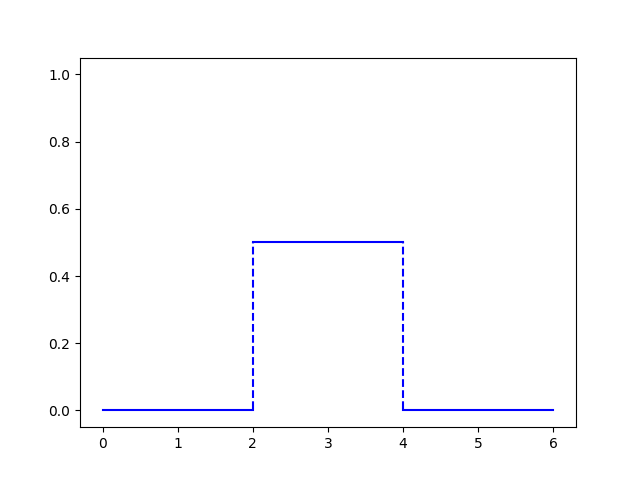
\includegraphics[width=0.45\textwidth]{uniformna}
		\caption{Uniformna porazdelitev na intervalu $[2, 4]$.}
	\end{figure}
		}
	\item {
		Zgoraj smo se že srečali s porazdelitvijo inteligenčnega količnika. To porazdelitev imenujemo \textbf{normalna} (ali \textbf{Gaussova}) \textbf{porazdelitev}, njena gostota verjetnosti pa je funkcija:
		\begin{equation}
			\N^{\mu, \sigma}(x) = \frac{1}{\sqrt{2\pi\sigma^2}}\cdot e^{-\frac{(x-\mu)^2}{2\sigma^2}},
		\end{equation}
		kjer je $\mu$ srednja vrednost (vrednost, kjer ima normalna porazdelitev maksimum - pri inteligenčnem količniku je $100$), $\sigma$ pa standardni odklon statistične populacije:
		\begin{equation}
			\sigma = \sqrt{\frac{\sum_{i=1}^N (x_i - \overset{\_}{x})^2}{N}},
		\end{equation}
		kjer je $x_i$ i-ta spremenljivka populacije, $\overset{\_}{x}$ povprečje populacije in $N$ velikost populacije (pri inteligenčnem količniku je $\sigma = 15$). Omenimo še pojem variance. \textbf{Varianca} je kvadrat standardnega odklona: $\sigma^2$.
	}
	\item {
		Kot zadnji primer si oglejmo porazdelitev \textbf{Gaussovske mešanice}. Gostota te porazdelitve je podana kot:
		\begin{equation}
			p(x) = \sum_{i=1}^n n(i) \cdot \N_i^{\mu_i, \sigma_i}(x),
		\end{equation}
		kjer so $\N_i^{\mu_i, \sigma_i}$ normalne porazdelitve, $n(i)$ pa taka pozitivna realna števila med $0$ in $1$, da velja: $\sum_{i=1}^n n(i) = 1$. Poglejmo si konkreten primer:
		\begin{equation}\label{gaussian-mixture-model}
			p(x) = \frac{1}{3} \cdot (\N^{-7,1}(x) + \N^{0,2}(x) + \N^{10,3}(x)).
		\end{equation}
		\begin{figure}[!ht]
			\centering
			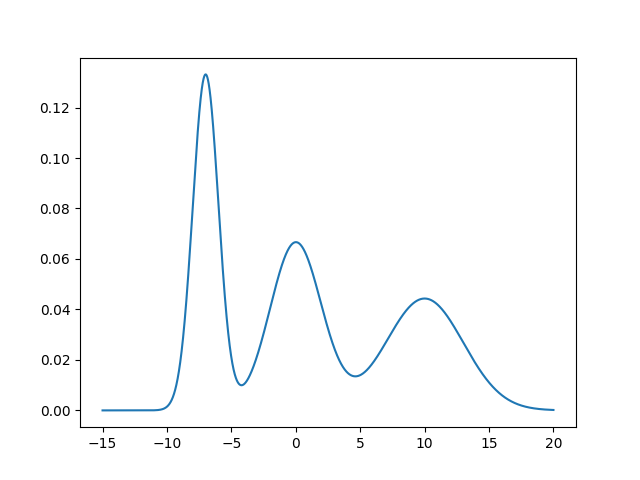
\includegraphics[width=0.5\textwidth]{gauss-mixture}
			\caption{Porazdelitev Gaussovske mešanice \eqref{gaussian-mixture-model}}
		\end{figure}
	}
\end{enumerate}
\end{zgled}
	

Za zaključek pregleda osnovnih pojmov omenimo še, da bomo v nadaljevanju velikokrat govorili o porazdelitvi in v mislih imeli gostoto verjetnosti te porazdelitve.

\section{Divergenca glede na gostoto verjetnosti}

Divergenca ima lahko več pomenov. V analizi se ta pojem uporablja pri obravnavanju zaporedij in vrst (takrat govorimo o konvergenci in divergenci zaporedja oz. vrste). V tem poglavju bomo predstavili še drugi pomen divergence.

\subsection{Definicija divergence}

Najprej navedimo motivacijski zgled za uporabo divergence.

\begin{zgled}
	V podjetju s proizvodnjo na tekočem traku nas zadolžijo za oskrbo tekočega traku. Naša naloga je, da sporočimo napako, ko jo zaznamo. Napake lahko zaznamo z odstopanjem izhodnih podatkov (npr. temperatura, vibracije, glasnost, itd.).

	Nastane problem: kako sploh primerjati trenutne podatke z optimalnimi in kdaj je odstopanje podatkov dovolj veliko? Potrebujemo metodo, s pomočjo katere bomo lahko primerjali razliko med dvema množicama podatkov. Poleg tega moramo z zagotovostjo trditi, da je prišlo do napake. Pomagamo si z divergenco.
\end{zgled}

Divergenca je torej merilo za razliko med dvema statističnima vzorcema (vzorca si lahko predstavljamo kot dve porazdelitvi). Navedimo formalno definicijo.

\begin{definicija}
	Naj bo $S$ prostor vseh verjetnostnih porazdelitev na istem definicijskem območju (tj. porazdelitve z istimi nosilci - na istem območju niso enake 0). \textbf{Divergenca} na $S$ je funkcija $D(\cdot \| \cdot): S \times S \rightarrow \mathbb{R}$, tako da velja:
	\begin{enumerate}
		\item $D(p \| q) \geq 0$ za vsaka $p, q \in S$,
		\item $D(p \| q) = 0 \Leftrightarrow p = q$.
	\end{enumerate}
	\textbf{Dualna divergenca} $D^\ast$ je definirana kot $D^\ast(p \| q) = D(q \| p)$.
\end{definicija}

Divergenca ni nujno simetrična in zanjo ne velja trikotniška neenakost, zato ne moremo enačiti pojmov divergenca in metrika.



\subsection{Divergenca univariatnih porazdelitev}

Definiranih je več različnih divergenc. Vsaka divegenca ima neke koristne lastnosti (npr. ena divergenca je bolj občutljiva glede na srednje vrednosti porazdelitev, tj. bo velika, ko se bodo srednje vrednosti razlikovale; spet druga divergenca je bolj občutljiva na varianco porazdelitev).

Renyi divergenci se bomo posvetili v naslednjem poglavju. Brez dokazov, da je to res divergenca, navedimo še nekaj ostalih primerov divergenc. Navedimo samo formule za zvezne spremenljivke, saj je formula za diskretne spremenljivke analogna (namesto integrala uporabimo vsoto).

\begin{zgled}
	\leavevmode
	\begin{enumerate}
		\item \textbf{Kullback-Leiblerjeva divergenca}:
		\begin{equation}
			D_{KL}(p \| q) = \int_\Omega p(x) \cdot \log\Big(\frac{p(x)}{q(x)}\Big) \  dx,
		\end{equation}
		kjer sta $p$ in $q$ porazdelitvi z definicijskim območjem $\Omega$.
		\item \textbf{f-divergenca}:
		To je družina divergenc, generirana s funkcijami $f$, za katere velja:
		\begin{itemize}
			\item $f$ konveksna na $\mathbb{R}^+$,
			\item $f(1) = 0$.
		\end{itemize}
		Elementi te družine so oblike:
		\begin{equation}
			D_f(p \| q) = \int_\Omega p(x) \cdot f\Big(\frac{p(x)}{q(x)}\Big) \  dx,
		\end{equation}
		kjer sta $p$ in $q$ porazdelitvi definirani na definicijskem območju $\Omega$.
		\item \textbf{Hellingerjeva distanca}:
		\begin{equation}
			H^2(p, q) = 2 \int_\Omega \Big(\sqrt{p(x)} - \sqrt{q(x)}\Big)^2 \  dx,
		\end{equation}
		kjer sta $p$ in $q$ porazdelitvi definirani na definicijskem območju $\Omega$.
	\end{enumerate}
\end{zgled}

\subsection{Renyi divergenca}

Nekoliko podrobneje oglejmo \textbf{Renyi divergenco}. Omejili se bomo le na zvezne spremenljivke, saj je definicija za diskretne analogna.


\begin{definicija}
	Naj bosta $P$ in $Q$ porazdelitvi z definicijskim območjem $\Omega$, $p$ in $q$ po vrsti gostoti verjetnosti porazdelitev $P$ in $Q$ ter $\alpha > 0$, $\alpha \neq 1$. Tedaj je \textbf{Renyi divergenca} definirana kot:
	\begin{equation}
		D_{\alpha}(P \| Q)=\frac{1}{\alpha-1} \cdot \log \int_{\Omega} \Big(p(x)\Big)^{\alpha}\Big(q(x)\Big)^{1-\alpha}\  dx.
	\end{equation}
\end{definicija}

Dokazati moramo naslednji izrek:

\begin{izrek}
	Renyi divergenca je divergenca.
\end{izrek}

\begin{proof}
	Naj bo $S$ prostor gostot verjetnosti.
	Dokazati moramo:
	\begin{enumerate}
		\item $D(p \| q) \geq 0$ za vsaka $p, q \in S$,
		\item $D(p \| q) = 0 \Leftrightarrow p = q$.
	\end{enumerate}
	Najprej dokažimo, da je Renyi divergenca vedno pozitivna. Namesto $p(x)$ in $q(x)$ pišimo kar $p$ in $q$. Dokazati moramo:
	\begin{equation}
		\label{neenakost}
		\frac{1}{\alpha - 1}\log \int_\Omega p^\alpha q^{1-\alpha} \  dx \geq 0.
	\end{equation}
	Ločimo primere:
	\begin{itemize}
		\item $\alpha > 1$: ker je prvi faktor v neenakosti \ref{neenakost} pozitiven za $\alpha > 1$, je ekvivalentno dokazati, da
		\begin{equation*}
			\log \int_\Omega p^\alpha q^{1-\alpha}  dx \geq 0
		\end{equation*}
		oziroma
		\begin{equation*}
			\int_\Omega p^\alpha q^{1-\alpha}  dx \geq 1
		\end{equation*}
		oziroma
		\begin{equation*}
			\int_\Omega \Big(\frac{p}{q}\Big)^\alpha q \  dx \geq 1.
		\end{equation*}
		Uporabimo Jensenovo neenakost za konveksno funkcijo $\phi$:
		\begin{equation*}
			\phi(\int f(x) dx) \leq \int (\phi \circ f) (x) dx,
		\end{equation*}
		kjer izberemo funkcijo $\phi(t) = t^\alpha$:
		\begin{equation*}
			\int_\Omega \Big(\frac{p}{q}\Big)^\alpha q \  dx \geq \Big(\int_\Omega \frac{p}{q} q dx\Big)^\alpha = \Big(\int p dx\Big)^\alpha = 1,
		\end{equation*}
		kjer smo upoštevali, da je $\int_\Omega p dx = 1$ po definiciji gostote verjetnosti.
		\item $0 < \alpha < 1$: ker je prvi faktor v neenakosti \ref{neenakost} negativen za $0 < \alpha < 1$, je ekvivalentno dokazati, da
		\begin{equation*}
			\log \int_\Omega p^\alpha q^{1-\alpha}  dx \leq 0
		\end{equation*}
		oziroma
		\begin{equation*}
			0 < \int_\Omega p^\alpha q^{1-\alpha}  dx \leq 1
		\end{equation*}
		oziroma
		\begin{equation*}
			0 <\int_\Omega \Big(\frac{q}{p}\Big)^{1-\alpha} p \  dx \leq 1.
		\end{equation*}
		Uporabimo Jensenovo neenakost za konkavno funkcijo $\phi$:
		\begin{equation*}
			\phi(\int f(x) dx) \geq \int (\phi \circ f) (x) dx,
		\end{equation*}
		kjer izberemo funkcijo $\phi(t) = t^{1-\alpha}$:
		\begin{equation*}
			\int_\Omega \Big(\frac{q}{p}\Big)^{1-\alpha} p \  dx \leq \Big(\int_\Omega \frac{q}{p} p \ dx\Big)^{1-\alpha} = \int_\Omega q \ dx = 1,
		\end{equation*}
		kjer smo upoštevali, je $\int_\Omega q dx = 1$ po definiciji gostote verjetnosti.
	\end{itemize}
	Dokažimo še drugo točko, torej
	\begin{equation}\label{eq-ekvivalenca-renyi}
		\frac{1}{\alpha - 1}\log \int_\Omega p^\alpha q^{1-\alpha} \  dx = 0 \Leftrightarrow p = q.
	\end{equation}
	Najprej dokažimo implikacijo iz desne proti levi ($\Leftarrow$):
	\begin{equation*}
		\frac{1}{\alpha - 1}\log\int_\Omega \Big(\frac{p}{p}\Big)^\alpha p \  dx = \frac{1}{\alpha - 1}\log\int_\Omega p \  dx = \frac{1}{\alpha - 1}\log 1 = 0.
	\end{equation*}
	V drugo smer ($\Rightarrow$) naredimo kratek premislek. Izraz na levi strani ekvivalence \eqref{eq-ekvivalenca-renyi} bo enak $0$, ko:
	\begin{enumerate}
		\item $\alpha = 0$, kar je v protislovju s predpostavko, da je $\alpha > 0$,
		\item $p = q$, saj bo takrat \ \  $\log\int_\Omega p \ dx = \log 1 = 0$.
	\end{enumerate}
	Zadnja implikacija je dokazana površno, saj bi se lahko zgodilo tudi, da implikacija ($\Rightarrow$) iz 2. točke velja, če $p \neq q$. Zaključimo, da se to zaradi lastnosti gostot verjetnosti ne more zgoditi.
\end{proof}

Renyi divergenca ni definirana v $\alpha = 1$, a v tej točki poznamo njeno vrednost:

\begin{izrek}\label{div_v_1}
	Naj bo $D_\alpha(P \| Q)$ Renyi divergenca porazdelitev $P$ in $Q$. Tedaj velja:
	\begin{equation}
		\lim_{\alpha \rightarrow 1} D_\alpha(P \| Q) = \int_\Omega p(x) \cdot \log\Big(\frac{p(x)}{q(x)}\Big) \  dx,
	\end{equation}
	kjer je izraz na desni ravno \textbf{Kullback-Leiblerjeva} divergenca porazdelitev $P$ in $Q$, tj.
	\begin{equation}
		\lim_{\alpha \rightarrow 1} D_\alpha(P \| Q) = D_{KL} (P \| Q).
	\end{equation}
\end{izrek}

Dokažimo izrek \ref{div_v_1}:

\begin{proof}
	Izračunajmo limito $D_\alpha(P \| Q)$, ko gre $\alpha$ proti $1$.
	\begin{equation*}
		\lim_{\alpha \rightarrow 1} \frac{\log \int p(x)^{\alpha}q(x)^{1-\alpha}\  dx}{\alpha-1} = \mathquotes{\frac{0}{0}},
	\end{equation*}
	zato lahko uporabimo L'Hospitalovo pravilo:
	\begin{equation*}
		\lim_{x \rightarrow a} \frac{f(x)}{g(x)} = \lim_{x \rightarrow a} \frac{f'(x)}{g'(x)}.
	\end{equation*}
	Posebej izračunajmo odvoda števca in imenovalca. Odvod imenovalca je trivialen: $(\alpha - 1)' = 1$. Odvajajmo še števec:
	\begin{align*}
		&\frac{d}{d\alpha}\Big( \log \int_\Omega p(x)^{\alpha}q(x)^{1-\alpha}\  dx\Big) = \frac{1}{\int_\Omega p(x)^{\alpha}q(x)^{1-\alpha}\  dx} \quad  \frac{d}{d\alpha}\int_\Omega p(x)^{\alpha}q(x)^{1-\alpha}\  dx \overset{(\ast)}{=} \\ &\overset{(\ast)}{=} \frac{1}{\int_\Omega p(x)^{\alpha}q(x)^{1-\alpha}\  dx} \quad \int_\Omega \frac{\partial}{\partial\alpha}\Big(p(x)^{\alpha}q(x)^{1-\alpha}\  dx\Big) = \\ &= \frac{1}{\int_\Omega p(x)^{\alpha}q(x)^{1-\alpha}\  dx} \quad \int_\Omega \Big(p(x)^\alpha \cdot \log p(x) \cdot q(x)^{1 - \alpha} - p(x)^\alpha \cdot q(x)^{1 - \alpha} \cdot \log q(x)\Big)dx = \\ &= \frac{1}{\int_\Omega p(x)^{\alpha}q(x)^{1-\alpha}\  dx} \quad \int_\Omega p(x)^\alpha \cdot q(x)^{1 - \alpha} \cdot \log \frac{p(x)}{q(x)} \ \  dx,
	\end{align*}
	kjer smo pri $(\ast)$ upoštevali, da je $F(\alpha) = p(x)^\alpha \cdot q(x)^{1 - \alpha}$ zvezna funkcija. Če izračunamo limito kvocienta odvodov, dobimo:
	\begin{equation*}
		\lim_{\alpha \rightarrow 1} \frac{\int_\Omega p(x)^\alpha \cdot q(x)^{1 - \alpha} \cdot \log \frac{p(x)}{q(x)} \ \  dx}{\int_\Omega p(x)^{\alpha}q(x)^{1-\alpha}\  dx} = \frac{1}{\int_\Omega p(x)\  dx} \ \int_\Omega p(x) \cdot \log \frac{p(x)}{q(x)} \ \  dx.
	\end{equation*}
	Če upoštevamo, da $\int_\Omega p(x) \ \ dx = 1$, dobimo:
	\begin{equation*}
		\int_\Omega p(x) \cdot \log \frac{p(x)}{q(x)} \ \  dx
	\end{equation*}
	kar je po definiciji ravno Kullback-Leiblerjeva divergenca.
\end{proof}



\subsection{Renyi divergenca normalnih porazdelitev}

Kot zgled si poglejmo izračun Renyi divergence za nekaj normalnih porazdelitev. Podajmo jih z enačbami:

\begin{equation}\label{norm_porazd}
	\begin{aligned}
		\N_1^{0,1}(x) &= \frac{1}{\sqrt{2\pi}}\cdot e^{-\frac{x^2}{2}} \\
		\N_2^{5,1}(x) &= \frac{1}{\sqrt{2\pi}}\cdot e^{-\frac{(x-5)^2}{2}} \\
		\N_3^{0,5}(x) &= \frac{1}{5\sqrt{2\pi}}\cdot e^{-\frac{x^2}{50}} \\
		\N_4^{0,10}(x) &= \frac{1}{10\sqrt{2\pi}}\cdot e^{-\frac{x^2}{200}}.
	\end{aligned}
\end{equation}

kjer je $\N_i^{\mu_i, \sigma_i}$ gostota verjetnosti porazdelitve $P_i$. Za predstavo si oglejmo še grafe teh verjetnostnih porazdelitev:

\begin{figure}[!ht]
	\centering
	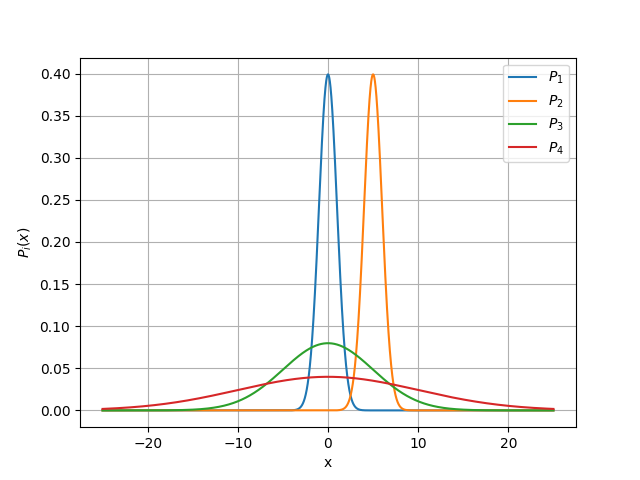
\includegraphics[scale=0.8]{normalne4}
	\caption{Normalne porazdelitve.}
\end{figure}

Brez simbolnega računanja si poglejmo divergenco med normalnimi porazdelitvami \eqref{norm_porazd}.

\begin{figure}[!ht]
	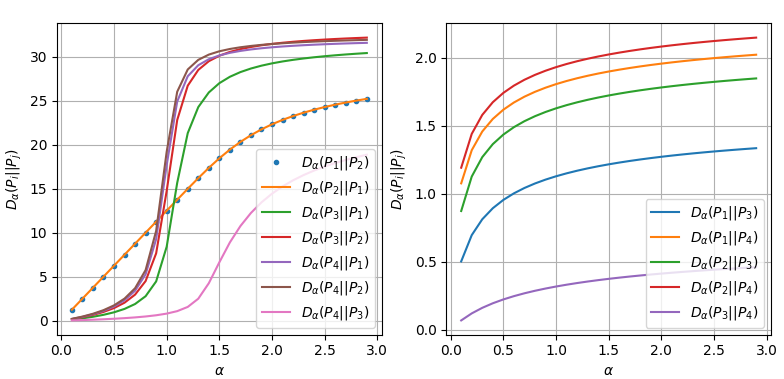
\includegraphics[scale=0.8]{divnorm}
	\caption{Divergence normalnih porazdelitev.}
	\label{divergence}
\end{figure}
\pagebreak
Na podlagi izračunov omenimo ugotovitvi:
\begin{enumerate}
	\item Opazimo, da bo vrednost Renyi divergence zelo velika, če bo varianca prve porazdelitve večja kot varianca druge porazdelitve in majhna, če bo varianca prve porazdelitve manjša kot varianca druge porazdelitve.
	\item Če je varianca porazdelitev $P_1$ in $P_2$ enaka, je Renyi divergenca simetrična, t.j. 
	\begin{equation*}
		D(P_1 \| P_2) = D^{\ast}(P_1 \| P_2) = D(P_2 \| P_1).
	\end{equation*}
\end{enumerate}

Če lahko sklepamo na podlagi Renyi divergence normalnih porazdelitev smo ugotovili, da na Renyi divergenco zelo vpliva razmerje med variancama prve in druge porazdelitve. Zaradi tega je lahko razlika med vrednostjo Renyi divergence in vrednostjo dualne Renyi divergence zelo velika.

Brez dokaza omenimo še, da translacija sistema ne vpliva na izračun Renyi divergence normalnih porazdelitev, to pomeni:
\begin{equation}
	D_\alpha\Big(\N^{\mu_1, \sigma_1}(x) \| \N^{\mu_2, \sigma_2}(x)\Big) = D_\alpha\Big(\N^{\mu_1, \sigma_1}(x - a) \| \N^{\mu_2, \sigma_2}(x - a)\Big),
\end{equation}
kjer je $a \in \mathbb{R}$.

\begin{opomba}
	Izračun divergenc in izris grafov sta bila narejena s programskim jezikom \texttt{Python3}.
\end{opomba}

\subsection{Numerično računanje Renyi divergence}

Kljub temu, da v definiciji divergence zahtevamo, da imata porazdelitvi ista nosilca oz. sta na istih območjih neničelni, se to v praksi pogostokrat ne obnese.

Prva težava je, da bi mogoče hoteli primerjati tudi porazdelitve, ki nimajo istih nosilcev. Vsako porazdelitev lahko razširimo na $\RR$ tako, da ji povsod, kjer ta ni definirana, priredimo vrednost 0. S tem sicer dobimo porazdelitvi z istim difinicijskim območjem, a nimata istih nosilcev. Seveda pa se poraja vprašanje, ali je sploh smiselno primerjati porazelitvi z različnima nosilcema? Na primer, ali je smiselno primerjati uniformno porazdelitev na intervalu $[0, 1]$ z uniformno porazdelitvijo na intervalu $[2, 3]$? Bralec naj to presodi sam.

Drugo težavo malce bolj analizirajmo, saj se pojavi tudi, ko imata porazdelitvi ista nosilca. Kot primer vzemimo normalni porazdelitvi. Gostota verjetnosti normalne porazdelitve je funkcija $\RR \rightarrow \RR^+$, torej bi morali pri Renyi divergenci dveh normalnih porazdelitev vedno dobiti rezultat v množici realnih števil.

Naj bosta $p$ in $q$ gostoti verjetnosti poljubnih realnih funkcij. Problem nastane v repih normalnih porazdelitev. Kljub temu, da je $p(x) > 0$ in $q(x) > 0$ za vsak $x \in \RR$, pride do numeričnih težav (deljenje z ničlo). Zakaj? Pride do podkoračitve (v neki točki nam računalnik zaokroži vrednost $p(x)$ na 0). Vpeljimo pojem konstante numerične ločljivosti.

\begin{definicija}
    \textbf{Konstanta numerične ločljivosti} je najmanjše pozitivno število, ki ga operacijski sistem še ne zaokroži na 0 (t.j. v operacijskem sistemu najmanjše predstavljivo število).
\end{definicija}

\begin{zgled}
    V 64-bitnem operacijskem sistemu je konstanta numerične ločljivosti enaka \\$\epsilon = 2,220446049250313 \cdot 10^{-16}$. Torej bodo vsa števila med 0 in $\epsilon$ zaokrožena na 0.
\end{zgled}

Predpostavimo, da operiramo s 64-bitni sistemom. Naj bo od zdaj naprej \begin{equation*}
    \epsilon = 2,220446049250313 \cdot 10^{-16}.
\end{equation*}

Torej, normalna porazdelitev $p$ bo neničelna le na intervalu $[x_1, x_2]$, kjer sta $x_1$ in $x_2$ rešitvi enačbe $p(x) = \epsilon$, za število $a$ na komplementu tega intervala pa bo $p(a)=0$. Analogno sklepamo za normalno porazdelitev $q$.

Zaradi takšnega zaokroževanja pride pri izračunu Renyi divergence do deljenja s številom 0. Spomnimo se formule za izračun Renyi divergence:
\begin{equation}
D_\alpha(p \| q) =
\begin{cases}
    \frac{1}{\alpha-1} \log \int_{\Omega} p(x)^{\alpha}q(x)^{1-\alpha}  dx&, \quad \alpha \neq 1 \\
    \quad \int_{\Omega} p(x) \log \frac{p(x)}{q(x)} dx&, \quad \alpha = 1
\end{cases}
\end{equation}
Najprej obravnavajmo težave pri $\alpha \neq 1$. Pride do deljenja z ničlo, ko je $q(x) = 0$ za nek $x$, ker je 
\begin{equation}
    q(x)^{1-\alpha} = q(x)\cdot\Big(\frac{1}{q(x)}\Big)^\alpha.
\end{equation}
Temu problemu se izognemo tako, da definiramo:
\begin{itemize}
    \item $\frac{0}{0}=0$,
	\item $\frac{a}{0}=\infty$ \ za $a>0$,
	\item $\log\infty = \infty$.
\end{itemize}
Če se torej zgodi, da so obe gostoti hkrati 0, ni težav. Ampak v trenutku, ko je $q(x) = 0$ in $p(x) \neq 0$, bo $D_\alpha(p \| q) = \infty$.

Prav tako se deljenje z 0 pojavi pri $\alpha = 1$. Poleg zgoraj definiranih pravil, s katerimi se izognemo težavam, definirajmo še:
\begin{itemize}
    \item $\log 0 = -\infty$.
\end{itemize}

Opazimo, da lahko kar hitro pridemo do rezultata $\infty$ oz. $-\infty$. Poglejmo, kaj bi lahko storili, da bi vedno dobili rezultat na intervalu $(-\infty, \infty)$. Moramo pa paziti, saj s tem postopkom nekoliko posegamo v same gostote verjetnosti in na koncu za gostoto verjetnosti $p$ ne bo več veljalo $\int_\Omega p(x) dx = 1$. Če pa bo to posegaje minimalno, kar je odvisno od primera do primera, pa lahko na pravilen način pridemo do rezultata na željenem intervalu $(-\infty, \infty)$.

\begin{opomba}
    \textbf{(dogovor)} Število $a$ je numerično enako $0$ oziroma numerično ničelno, če je enako $0$ ali če je $|a| < \epsilon$ (tedaj pride do podkoračitve).
\end{opomba}

Vzemimo poljubni gostoti verjetnosti $p, q$ in ju razširimo na $\RR$. Naj bo $m$ tako število, da velja:
\begin{equation*}
    \forall x_0 < m, \forall \delta > 0:
    \Big(p(x_0) < \epsilon \ \  \wedge \ \  q(x_0) < \epsilon\Big)
    \wedge
    \Big(p(m + \delta) \geq \epsilon \ \  \vee \ \  q(m + \delta) \geq \epsilon\Big),
\end{equation*}
t.j. $m$ je tako število, da sta gostoti verjetnosti numerično ničelni na intervalu $(-\infty, m)$ (zaradi podkoračitve) in $m$ je največje tako število. Vemo, da tako število obstaja, saj je $\lim_{x \rightarrow -\infty} p(x) = 0$ za poljubno gostoto verjetnosti $p$ (ploščina med $p$ in $x$-osjo je $1$). Naj bo $M$ tako število, da velja:
\begin{equation*}
    \forall x_0 > M, \forall \delta > 0:
    \Big(p(x_0) < \epsilon \ \  \wedge \ \  q(x_0) < \epsilon\Big)
    \wedge
    \Big(p(M - \delta) \geq \epsilon \ \  \vee \ \  q(M - \delta) \geq \epsilon\Big),
\end{equation*}
t.j. $M$ je tako število, da sta gostoti verjetnosti numerično ničelni na intervalu $(M, \infty)$ (zaradi podkoračitve) in $M$ je najmanjše tako število. Vemo, da tako število obstaja, saj je $\lim_{x \rightarrow \infty} p(x) = 0$ za poljubno gostoto verjetnosti $p$.

Na komplementu intervala $[m, M]$ bodo zaradi numerične ločljivosti obe gostoti enaki 0. Na intervalu $[m, M]$ pa definirajmo novi funkciji:
\[
f(x) := 
\begin{cases}
    p(x) &, \  p(x) > \epsilon \\
    \quad \epsilon &, \  p(x) \leq \epsilon
\end{cases}
\quad \quad \text{in} \quad \quad
g(x) := 
\begin{cases}
    q(x) &, \  q(x) > \epsilon \\
    \quad \epsilon &, \  q(x) \leq \epsilon
\end{cases}
\quad .
\]
Funciji $f$ in $g$ se od $p$ in $q$ razlikujeta le tam, kjer sta $p$ in $q$ zaradi podkoračitve enaka 0. Preveriti moramo le še, da je $\int_{[m,M]} f(x) dx \approx 1$ in $\int_{[m,M]} g(x) dx \approx 1$. To bo res, če bo skupna dolžina podintervalov na $[m, M]$, kjer sta $p, q < \epsilon$, majhna. Sedaj lahko naredimo aroksimacijo: $D_\alpha(p \| q) \approx D_\alpha(f \| g)$, kjer zagotovo ne pride do deljenja z 0. Kljub temu pa bodo te vrednosti zaradi deljenja z $\epsilon$ lahko zelo velike.

\begin{opomba}
    Kdaj lahko $\int_{[m,M]} f(x) dx$ zaokrožimo na 1, je odvisno od tega, kakšna napaka je za nas še zadovoljiva. Na primer, če je skupna dolžina podintervalov na $[m,M]$, kjer je $p(x) < \epsilon$, enaka 1000, se bo vrednost $\int_{[m,M]} f(x) dx$ absolutno razlikovala od 1 za približno $2,22 \cdot 10^{-13}$.
\end{opomba}
\pagebreak
\subsection{Divergenca bivariatnih in multivariatnih porazdelitev}

Do sedaj smo obravnavali divergenco univariatnih porazdelitev, torej gostota verjetnosti je bila funkcija ene spremenljivke (npr. P porazdelitev, $p: \RR \rightarrow \RR$ njena gostota verjetnosti). Kaj pa če gledamo porazdelitve v več dimenzijah? Za začetek si poglejmo zgled.

\begin{zgled}
    Poglejmo si zgled bivariatne normalne porazdelitve. Kot primer v vsakdanjem življenju lahko vzamemo npr. populacijo ljudi in hkrati gledamo višino in težo.
    \begin{figure}[!ht]
        \centering
        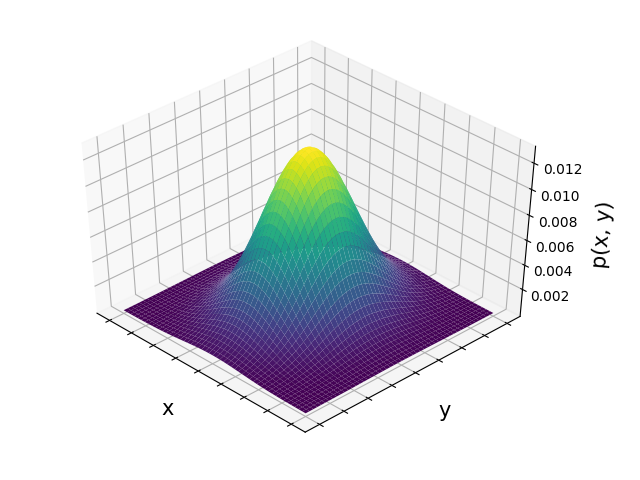
\includegraphics[width=\textwidth]{gauss-bivariate}
        \caption{Normalna porazdelitev v dveh dimenzijah.}
    \end{figure}
\end{zgled}

Izpustimo definicije in ostale primere porazdelitev, poglejmo raje, kako definiramo divergenco.
\pagebreak
Definicija divergence za bi- in multivariate porazdelitve sovpada z definicijo divergence za univariatne porazdelitve:
\begin{enumerate}
	\item $D(p \| q) \geq 0$ za vsaka $p, q \in S$, kjer je $S$ množica porazdelitev,
	\item $D(p \| q) = 0 \Leftrightarrow p = q$.
\end{enumerate}

Recimo, da gledamo porazdelitve v $n$ dimenzijah. Gostote verjetnosti teh porazdelitev bodo funkcije $p: \Omega \subseteq \RR^n \rightarrow \RR^+$. Divergence se torej na naraven način prevedejo za $n$-dimenzionalne porazdelitve. Poglejmo si to na primerih.

\begin{zgled}
    Naj bo $x=(x_1, x_2, \dots , x_n) \in \RR^n$. Naj bodo $p, q$ gostote verjetnosti z definicijskim območjem $\Omega \subseteq \RR^n$. Definicije divergenc razširimo na $n$ dimenzij:
	\begin{enumerate}
		\item \textbf{Kullback-Leiblerjeva divergenca}
		\begin{equation}
			D_{KL}(p \| q) = \idotsint\limits_\Omega p(x) \cdot \log\Big(\frac{p(x)}{q(x)}\Big) \  dx_1\dots dx_n.
		\end{equation}
		\item \textbf{f-divergenca}
		\begin{equation}
			D_f(p \| q) = \idotsint\limits_\Omega p(x) \cdot f\Big(\frac{p(x)}{q(x)}\Big) \  dx_1\dots dx_n.
		\end{equation}
		\item \textbf{Hellingerjeva distanca}
		\begin{equation}
			H^2(p, q) = 2 \cdot \idotsint\limits_\Omega \Big(\sqrt{p(x)} - \sqrt{q(x)}\Big)^2 \  dx_1\dots dx_n.
		\end{equation}
		\item \textbf{Renyi divergenca}
		\begin{equation}
			D_{\alpha}(p \| q)=\frac{1}{\alpha-1} \cdot \log \Bigg(\idotsint\limits_\Omega \Big(p(x)\Big)^{\alpha}\Big(q(x)\Big)^{1-\alpha}\  dx_1\dots dx_n\Bigg), \quad \quad \alpha \neq 1.
		\end{equation}
	\end{enumerate}
\end{zgled}

\subsection{Praktična uporaba}

Divergenca glede na gostoto verjetnosti je zelo uporabna v praktičnih problemih, ko glede na set podatkov naredimo oceno gostote verjetnosti z Gaussovimi jedri (angl. Gaussian kernel density estimation).

V splošnem bomo hoteli izračunati divergenco med dvema statističnima vzorcema. Skoraj nikoli divergence ne računamo analitično, saj pri obdelavi podatkov nimamo podane gostote verjetnosti teh podatkov eksplicitno in simbolno. Divergenco bomo izračunali z uporabo histogramov vzorcev ali pa z uporabo ocenjevalcev za gostoto verjetnosti.

\section{Predstavitev podatkov vzorca}

Naredimo preskok iz teorije v prakso. Imamo dva vzorca podatkov in želimo izračunati divergenco med njima. Pojavi se problem, saj ne vemo, kateri porazdelitvi ustrezata dana vzorca, torej nimamo teoretičnih gostot vertjetnosti. Poiskati želimo približek za gostoto verjetnosti. To naredimo z vpeljavo histogramov ali z vpeljavo različnih ocenjevalcev za gostoto verjetnosti.

\subsection{Histogram}\label{pog-histogram}

Naj bo $S$ množica podakov. Razdelimo interval $[\min(S), \max(S)]$ na $n \in \mathbb{N}$ intervalov z dolžino večjo od 0:
\[
[\min(S), \max(S)] = [a_0, a_1) \cup [a_1, a_2) \cup \ldots \cup [a_{n-2}, a_{n-1}) \cup [a_{n-1}, a_n].
\]
Omenimo, da $\min(S) = a_0$ in $\max(S) = a_n$. Naj bo
\[
    N: \{ 0, \ldots, n-1 \} \rightarrow \mathbb{N}
\]
funkcija s predpisom:
\[
N(i) = \sum_{x \in S} \delta_i(x),
\]
kjer je
\[
    \delta_i(x) =
    \begin{cases}
        1, \quad x \in [a_i, a_{i+1}) \\
        0, \quad \text{sicer}
    \end{cases}.    
\]
Če je $i = n - 1$, je v pogoju pri $\delta_{n-1}$ interval zaprt. Funkcija $N$ torej prešteje, koliko elementov iz $S$ je znotraj intervala $[a_i, a_{i+1})$.
\pagebreak
\begin{definicija}
    \textbf{Histogram} je funkcija $H: \mathbb{R} \rightarrow \mathbb{N}$ s predpisom:
    \begin{equation}
        H(x) =
        \begin{cases}
            \ N(i)&, \quad \exists i \in \{ 0, \ldots, n-1\} \ni: x \in [a_i, a_{i+1}) \\
            \quad 0&, \quad sicer 
        \end{cases},
    \end{equation}
    kjer v pogoju pri $i=n-1$ dopuščamo zaprti interval.
\end{definicija}

Pri obdelavi podatkov je bolj kot zgornja različica histograma uporabna naslednja:

\begin{definicija}
    \textbf{Normalizirani histogram} množice podatkov $S$ je funkcija $h: \mathbb{R} \rightarrow \mathbb{R}_+$ s predpisom:
    \begin{equation}
        h(x) =
        \begin{cases}
            \frac{N(i)}{|S|\cdot (a_{i+1} - a_i)}&, \quad \exists i \in \{ 0, \ldots, n-1\} \ni: x \in [a_i, a_{i+1}) \\
            \quad\quad 0&, \quad sicer 
        \end{cases},
    \end{equation}
    kjer v pogoju pri $i=n-1$ dopuščamo zaprti interval.
\end{definicija}

\begin{opomba}
    Normalizirani histogram ima lastnost: $\int_\mathbb{R} h(x) dx = 1$.
\end{opomba}

Poglejmo si zgled histograma in razliko med histogramom in normaliziranim histogramom.

\pagebreak
\begin{zgled}
    $S_0 = \{1,1.3,1,2.5,3,3.5,3.6,4,4.1,4.2,5\}$. \\
    $[\min(S_0), \max(S_0)]$ razdelimo na 4 podintervale: $[1,2), [2,3), [3,4), [4,5]$.
    Poglejmo, kako izgledata histogram in normaliziran histogram (slika \ref{hist-zgled}).
    \begin{figure}[!h]
        \begin{subfigure}{0.49\textwidth}
            \centering
            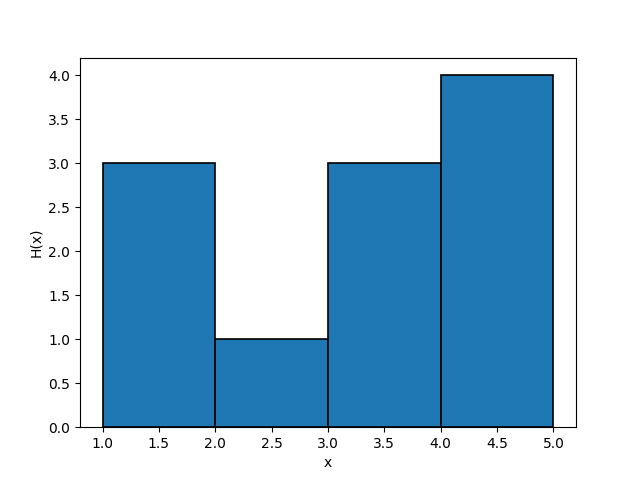
\includegraphics[scale=0.47]{histogram-zgled.png}
        \end{subfigure}
        \begin{subfigure}{0.49\textwidth}
            \centering
            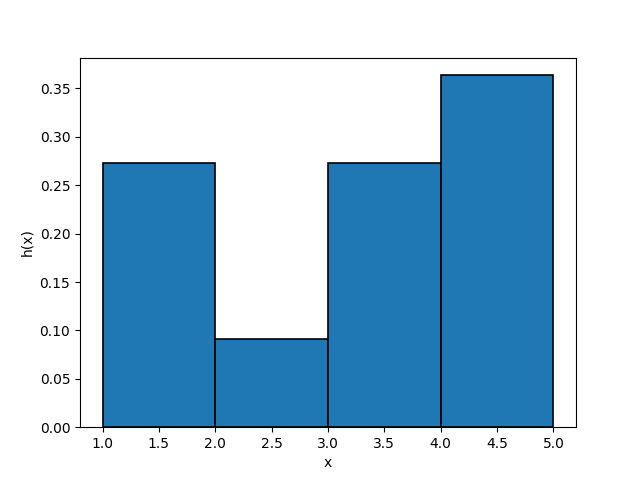
\includegraphics[scale=0.47]{histogram-norm-zgled.png}
        \end{subfigure}
        \caption{Na levi je (navaden) histogram, na desni pa normaliziran histogram vzorca $S_0$. Oblika je ista, razlika je v skali na y-osi.}
        \label{hist-zgled}
    \end{figure}
\end{zgled}

Od zdaj naprej bomo enačili pojma histogram in normaliziran histogram, z obema pa bomo v mislih imeli normaliziran histogram.

V zgledu opazimo, da histogram grafično ni podan kot funkcija. Opišimo  grafičen prikaz histogramov.

\pagebreak
\subsection{Grafični prikaz histogramov}

Histogram je odsekoma konstantna funkcija, kar je razvidno iz definicije ($h(x)$ je konstantna na vsakem intervalu $[a_i, a_{i+1})$). Zato si histogram lahko predstavljamo kot množico pravokotnikov, ki jim pravimo \textbf{stolpci} (angl. bins) histograma.

Naj bo na intervalu $[a_{i}, a_{i+1}), i \in \{0,\ldots,n-1\}$ i-ti stolpec oziroma stolpec i histograma, torej ima histogram $n$ stolpcev. Stolpec i ima širino $w_i = a_{i+1} - a_{i}$. Če so intervali enako dolgi, imajo vsi stolpci isto širino $w$. To širino lahko tudi izračunamo:
\begin{equation}\label{sirina_stevilo}
    w = \frac{\max(S)-min(S)}{n} = \frac{a_n - a_0}{n},
\end{equation}
kjer je n število stolpcev histograma.

Višina i-tega stolpca $h_i$ pa je vrednost funkcije $h$ v poljubni točki znotraj intervala \\ $[a_{i}, a_{i+1})$, torej:
\begin{equation}
    h_i = h(x) \quad \text{za} \quad \forall  x \in [a_{i}, a_{i+1}].
\end{equation}

Zgornji način predstavitve histograma ni uporaben le grafično, temveč tudi računsko. Namesto integrala funkcije $h$ lahko izračunamo vsoto ploščin stolpcev, da dokažemo, da je ploščina histograma enaka 1. Numerično se nam bo to izplačalo, saj je numerično integriranje bolj zahtevno kot računanje osnovnih operacij. Enako velja za izračun divergence, kjer uporabimo integracijo.
\pagebreak
\subsection{Optimalno število stolpcev histograma}

Recimo, da ima množica $S$ porazdelitev $P$. Naj bo $p$ gostota verjetnosti te porazdelitve, $h_n$ pa histogram množice $S$ z $n$ stolpci. Velja:
\begin{equation}
    \lim_{\begin{smallmatrix} |S| \to \infty \\ n \to \infty \end{smallmatrix}} h_n(x) = p(x) \quad \text{za} \quad \forall x \in S.
\end{equation}
Histogram je torej lahko ocena gostote verjetnosti množice $S$.

V nobenem vzorcu nimamo na voljo $\infty$ podatkov, zato moramo paziti na izbiro števila stolpcev histograma. Če je $n>|S|$, bo najmanj en stolpec prazen (oz. bo imel višino 0), torej bo to lahko zelo slab približek za gostoto verjetnosti (npr. normalna porazdelitev je povsod večja od 0). Druga skrajnost je, ko izberemo premalo stolpcev in tako izgubimo podatke o porazdelitvi (moduse, če jih ima vzorec več).


\begin{zgled}
Vzemimo množico $S_0 = \{1,1.3,1,2.5,3,3.5,3.6,4,4.1,4.2,5\}$. Poglejmo si histograme ob različni izbiri števila stolpcev.
\begin{figure}[!h]
    \centering
    \begin{subfigure}{0.3\textwidth}
        \centering
        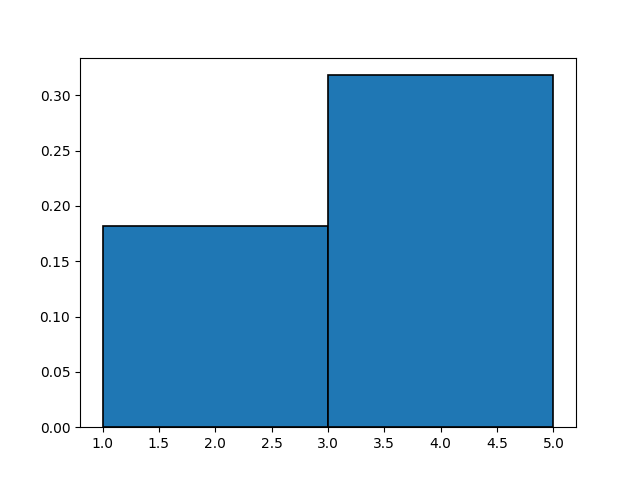
\includegraphics[scale=0.29]{hist-2bina.png}
        \caption{$n=2$}
        \label{2-bina}
    \end{subfigure}
    \begin{subfigure}{0.3\textwidth}
        \centering
        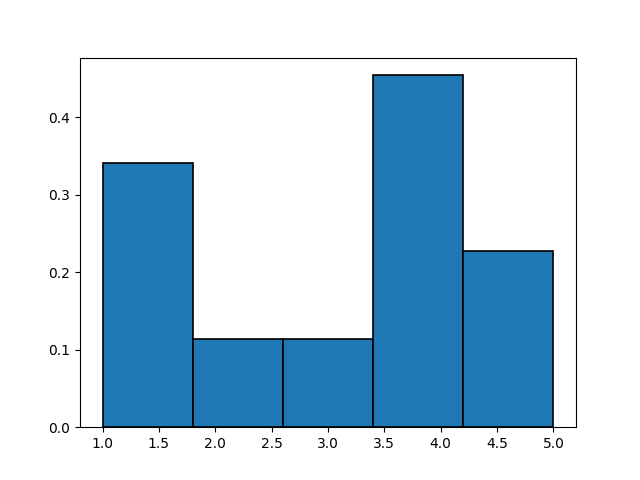
\includegraphics[scale=0.29]{hist-5binov.png}
        \caption{$n=5$}
        \label{5-binov}
    \end{subfigure}
    \begin{subfigure}{0.3\textwidth}
        \centering
        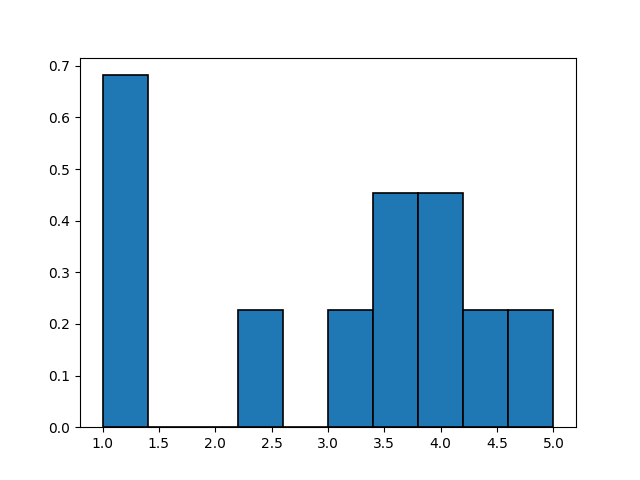
\includegraphics[scale=0.29]{hist-10binov.png}
        \caption{$n=10$}
        \label{10-binov}
    \end{subfigure}
    \caption{Histogrami z različnimi števili stolpcev.}
\end{figure}

V primeru \ref{2-bina} smo izbrali premalo stolpcev, s čimer lahko zgrešimo pomembne lastnosti množice $S$. V primeru \ref{10-binov} pa smo izbrali preveč stolpcev, s čimer dobimo prazne stolpce.
\end{zgled}

Obstaja veliko izbir za optimalno število stolpcev. Naštejmo jih. Za vse izbire naj bo $S$ vzorec in $m = |S|$ moč vzorca.

\pagebreak

\subsubsection{Korenska izbira}
Pri tej izbiri optimalno število stolpcev histograma izračunamo po naslednji formuli:
\begin{equation}
    n = \big\lceil \sqrt{m}\  \big\rceil.
\end{equation}
Izračunamo torej kvadratni koren od števila podatkov v vzorcu in zaokrožimo to število na najmanjše celo število, ki je večje od dobljenega korena.

% preveri alternativo za sklanjanje za Rice.
% PRAVILNO: Riceovo - mi ni všeč
% Kaj, ce je Rice bila zenska? Zaenkrat se izognem sklanjanju
% \subsubsection{Riceovo pravilo}
\subsubsection{Rice}
Pri tej izbiri optimalno število stolpcev za histogram izračunamo na naslednji način:
\begin{equation}
    n = \big\lceil \sqrt[3]{m}\  \big\rceil.
\end{equation}

\subsubsection{Sturges}
Pri tej izbiri optimalno število stolpcev izračunamo po naslednji formuli:
\begin{equation}
    n = \big\lceil \log_2{m}\  \big\rceil + 1.
\end{equation}
Ta formula je zelo varčna, saj logaritem narašča zelo počasi. Medtem ko bo pri korenski izbiri in 10000 podatkov optimalno število stolpcev 100, bo pri Sturgesovi formuli število stolpcev enako 11.

Vse tri do zdaj naštete izbire delujejo zelo naivno, saj upoštevajo le velikost vzorca, ne pa ostalih njegovih lastnosti, npr. variance. Kljub temu pa se izkaže, da te metode zelo dobro konkurirajo z ostalimi, če gledamo lepe porazdelitve, npr. normalne porazdelitve. Težava so bolj kompleksne porazdelitve, ki imajo visoke repe in so na eni strani omejene. Pri teh hitro dobimo premalo stolpcev in moramo nujno upoštevati še kakšno drugo lastnost, ne le velikosti vzorca.

\pagebreak
Poglejmo si sedaj še izbiri, ki upoštevata bolj specifične lastnosti vzorca. Ti dve formuli sicer vrneta optimalno širino stolpca, a zlahka iz tega podatka dobimo optimalno število stolpcev (glej formulo \eqref{sirina_stevilo}). 

\subsubsection{Scoot}
Formula Scoot poleg velikosti vzorca upošteva še njegov standardni odklon $\sigma$:
\begin{equation}
    h = 3,49 \cdot \sigma \cdot m^{-1/3}.
\end{equation}

\subsubsection{Freedman-Diaconis}
Ta izbira prav tako uporabi še dodatno lastnost poleg velikosti vzorca, in sicer medkvartilno razdaljo vzorca $IQR$ (angl. \textit{interquartile range}), to je razlika med zgornjim in spodnjim kvartilom. 
\begin{equation}
    h = 2 \cdot IQR \cdot m^{-1/3}.
\end{equation}

Ker smo že sproti opisali izbire, primer izpustimo. Omenimo pa, da sta zadnji dve metodi v splošnem najboljši, saj poleg velikosti vzorca upoštevata še dodatne lastnosti vzorca, poleg tega pa je izračun variance in medkvartilne razdalje hiter, zato metodi nista časovno potratni.
\pagebreak
\subsection{Enakovredni stolpci}

Do sedaj smo obravnavali samo stolpce, ki so imeli enako širino. Kaj pa, če je mogoče optimalna izbira taka, da stolpci niso enako široki? Eden od takih načinov je vpeljava enakovrednih stolpcev.

\begin{definicija}
    Naj bo $S$ množica podatkov. Naj bo $h$ histogram z $n$ stolpci, $n < |S|$, zgrajen glede na podatke iz $S$. Histogram ima \textbf{enakovredne stolpce}, če je v vseh stolpcih "približno enako" število podatkov.
\end{definicija}

\begin{figure}[!h]
    \centering
    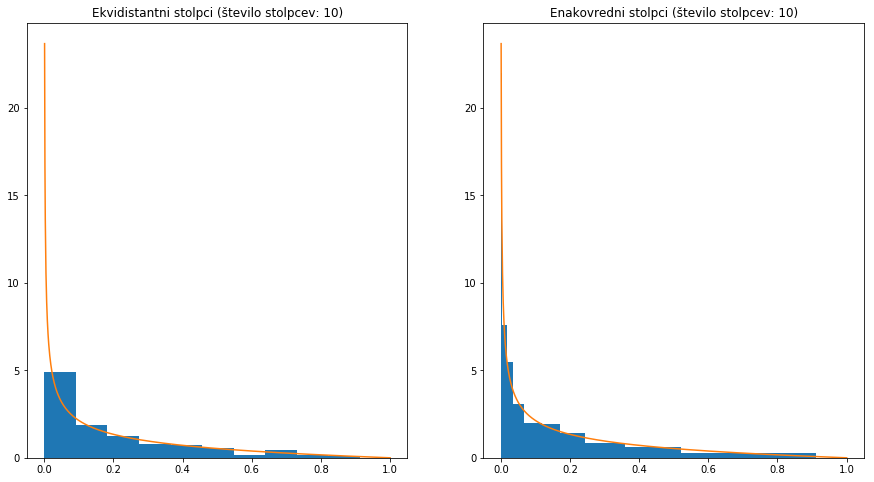
\includegraphics[width=\textwidth]{ekvikvan.png}
    \caption{Primerjava med histogramom z enako širokimi stolpci in histogramom z enakovrednimi stolpci za beta porazdelitev ($\alpha = 0.5$, $\beta = 2$). Vidimo, da se ob istem številu stolpcev veliko bolj prilegajo enakovredni stolpci}
\end{figure}

V zgornji definiciji smo uporabili besedno zvezo "približno enako", ker ni nujno, da je število $|S|$ deljivo s številom $n$. Pri konstrukciji takega histograma pa se temu problemu lahko izognemo recimo tako, da v zadnji stolpec damo toliko podatkov, kolikor je ostanek pri deljenju števila $|S|$ z $n$. Najprej opišimo, kako konstruiramo takšen histogram, nato pa si bomo to pogledali na zgledu.

\subsubsection*{Konstrukcija histograma z enakovrednimi stolpci}

Naj bo $S = \{x_1, x_2, \ldots, x_m\}$ množica podatkov. Konstruirati želimo histogram z $n$ stolpci. Ta histogram bo imel enakovredne stolpce, če bo v vsakem stolpcu $\lfloor m/n \rfloor$ podatkov (razen v zadnjem stolpcu, če število $m$ ni deljivo z $n$ - v tem primeru bomo dobili $n+1$ stolpcev). Potrebujemo meje stolpcev histograma. Enkrat, ko bomo imeli meje, bomo lahko zlahka dobili tudi višine.

Recimo, da je $S$ naraščajoče urejena, sicer pa jo tako uredimo. Naj bo $X$ prazen seznam, v katerega bomo vstavljali meje stolpcev. Prva meja je očitna: $S(1)$, ki je tudi minimalna vrednost množice $S$. Vstavimo torej $S(1)$ v seznam X.

Naj bo $k = \lfloor m/n \rfloor$. v 1. koraku naj bo $S_1$ kopija urejene množice brez prvih $k$ elementov. Nato v seznam $X$ dodamo najmanjši element nove množice $S_1$. Tako bosta v množici $X$ elementa $S(1)$ in $S_1(1)$. V tem stolpcu bo torej ravno $k$ elementov (element $S_1(1)$ bo ležal v naslednjem stolpcu).

Postopek ponavljamo, dokler ni v kopiji množice $S$ manj kot $k$ elementov. Tedaj v seznam $X$ dodamo zadnji, največji element množice $S$.

Višine dobimo tako, da preštejemo število podatkov v posameznem stolpcu, in to število deljimo z $m\cdot w$, kjer je $w$ širina stolpca.

\begin{zgled}
    Vzemimo $S = \{-17, -13, -9, -8, -6, -5.5, 0, 5.5, 6, 9, 10, 10.5, 11, 12\}$, $|S| = 14$. Želimo dobiti 4 enakovredne stolpce. Na začetku je v $X$ najmanjši element $S$, torej $X = [-17]$. Naš $k$ bo enak $\lfloor 14/4\rfloor = 3$. Nadaljujemo po korakih:
    \begin{enumerate}
        \item Iz $S$ odstranimo prve 3 elemente: $S_1 = \{-8, -6, -5.5, 0, 5.5, 6, 9, 10, 10.5, 11, 12\}$. Najmanjšega iz $S_1$ damo v $X$: $X = [-17, -8]$.
        \item IZ $S_1$ odstranimo prve 3 elemente: $S_2 = \{0, 5.5, 6, 9, 10, 10.5, 11, 12\}$. V $X$ dodamo najmanjšega: $X = [-17,-8,0]$.
        \item $S_3 = \{9, 10, 10.5, 11, 12\}$, $X = [-17,-8,0,9]$.
        \item $S_4 = \{11, 12\}$, $X = [-17,-8,0,9,11]$.
        \item V $S_4$ imamo samo dva elementa, zato v $X$ dodamo največjega: $X = [-17,-8,0,9,11,12]$
    \end{enumerate}
    Dobimo torej meje stolpcev $X=[-17,-8,0,9,11,12]$. Višine dobimo tako, da v vsakem stolpcu preštejemo število podatkov in to število deljimo z $14\cdot w$, kjer je $w$ širina stolpca.

    \begin{figure}[!h]
        \centering
        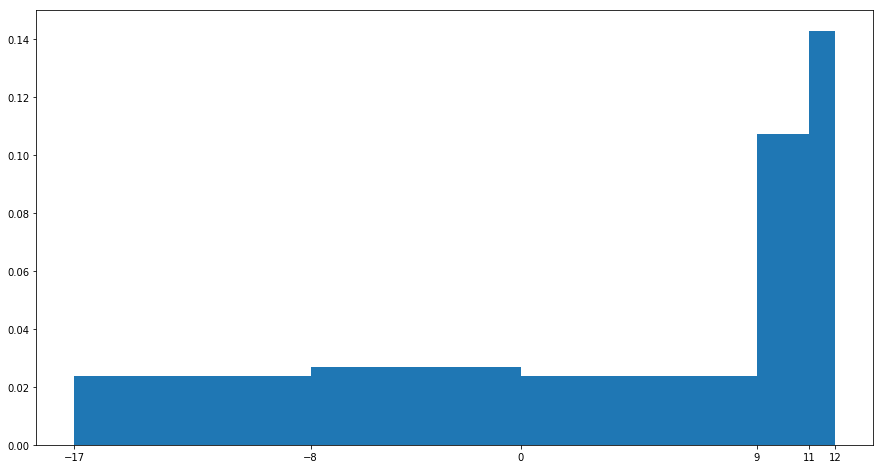
\includegraphics[width=\textwidth]{eqBinsZgled.png}
        \caption{Histogram množice $S$ z enakovrednimi stolpci. Zadnji stolpec vsebuje le 2 podatka, ostali pa 3.}
    \end{figure}

\end{zgled}
\pagebreak
\subsection{Ocena gostote verjetnosti z jedrom}
Opišimo še nekoliko drugačen pristop za predstavitev podatkov. Najprej pa moramo povedati, kaj sploh mislimo z besedo "jedro".
\begin{definicija}
    \textbf{Jedro} je nenegativna realna integrabilna funkcija $K$ z lastnostima:
    \begin{itemize}
        \item $\int_{-\infty}^\infty K(x) \  dx = 1 \quad$ in
		\item $K(-x) = K(x), \quad \forall x \in \mathbb{R} \quad$ (simetrija).
    \end{itemize}
\end{definicija}

\begin{figure}[!h]
    \centering
    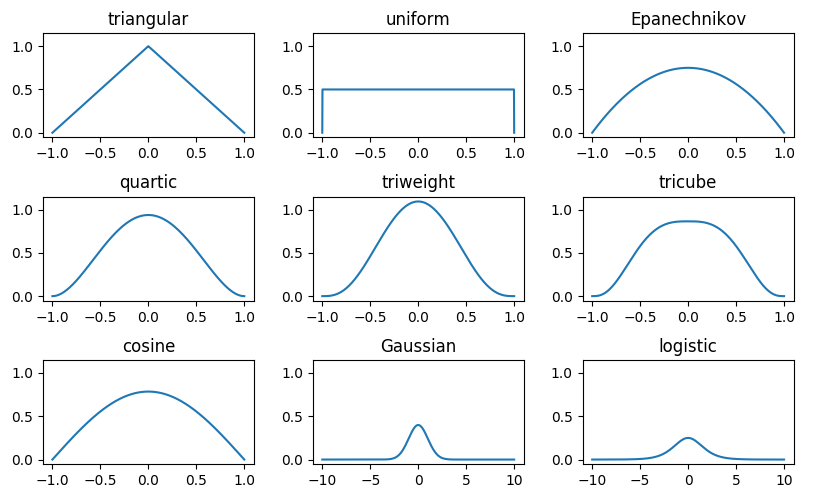
\includegraphics[width=\textwidth]{jedra.png}
    \caption{Nekaj primerov jeder.}
    \label{jedra}
\end{figure}

Ideja ocenjevanja gostote verjetnosti z jedri (angl. \textit{kernel density estimation}) je, da na vsako točko v vzorcu obesimo jedro, ki ga vnaprej določimo, nato pa ta jedra seštejemo in rezultat normiramo. Ker so jedra nenegativna, bo torej pridobljena funkcija ustrezala definiciji gostote verjetnosti.
\begin{definicija}
    \textbf{Ocena gostote verjetnosti z jedrom} je neparametričen način ocenjevanja gostote verjetnosti. Naj bo $K$ jedro in $X = \{x_1,\ldots,x_n\}$ množica podatkov.  Ocena gostote verjetnosti z jedrom $K$ množice $X$ je funkcija, definirana kot:
    \begin{equation}
        f_h(x) = \frac{1}{n\cdot h} \  \sum_{i=1}^n K\Big(\frac{x - x_i}{h}\Big),
    \end{equation}
    kjer je $h$ parameter glajenja, imenovan "bandwidth". % bandwidth == pasovna širina?? mislim da ne
\end{definicija}

Parameter $h$ močno vpliva na končno oceno. Če je $h$ premajhen, lahko dobimo močno oscilirajočo funkcijo, ob preveliki izbiri $h$ pa lahko izgubimo pomembne podatke o porazdelitvi. Če potegnemo vzporednico s podpoglavjem o histogramih, lahko rečemo, da $h$ igra podobno vlogo kot izbira optimalnega števila stolpcev pri histogramih. V optimizacijo paramtra $h$ se ne bomo poglabljali, ponavadi pa ga izračunamo kot:
\begin{equation}
    h = \sigma(X) \cdot \Big(\frac{4}{3|X|}\Big)^{1/5},
\end{equation}
kjer je $\sigma(X)$ standardni odklon množice podatkov $X$.

Pri ocenjevanju gostote verjetnosti z Gaussovim jedrom uporabljamo Gaussovo jedro (slika \ref{jedra}). To je normalna porazdelitev s srednjo vrednostjo 0 in varianco 1, torej:
\begin{equation}
	K(x) = \frac{1}{\sqrt{2\pi}}e^{-\frac{1}{2}x^2}.
\end{equation}
Ocenjevanje gostote verjetnosti z Gaussovim jedrom smo izpostavili, ker je zelo pogost. Poleg tega je zelo dobra ocena pri porazdelitvah s trebuhi (npr. normalna porazdelitev, Rayleigh porazdelitev, ...). Je pa ta metoda zelo slaba pri porazdelitev s končnimi nosilci (npr. uniformna podrazdelitev), saj zaradi neomejenosti definicijskega območja Gaussovega jedra funkcija, ki jo dobimo z oceno, preseže ta nosilec.

\begin{figure}[!h]
    \centering
    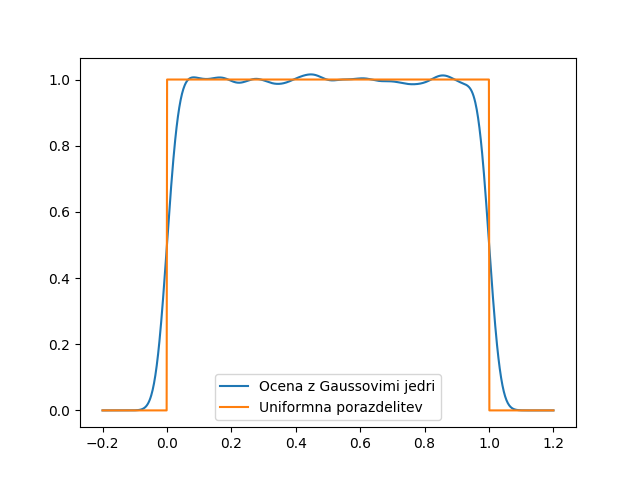
\includegraphics[width=0.45\textwidth]{gaussVSuniform.png}
    \caption{Vidi se, da ocena z Gaussovimi jedri preseže nosilec uniformne porazdelitve.}
\end{figure}
\pagebreak
Predstavili smo dva načina predstavitve podatkov. Obe načina predstavitve imata svoje prednosti in slabosti. Predstavitev s histogrami je zelo kompaktna, poleg tega pa histogram nikoli ne bo segal ven iz nosilca porazdelitve, saj je omejen s podatkovno množico. Pri ocenjevanju gostote verjetnosti z jedri se pa lahko zelo dobro približamo porazdelitvi, ki jo podatki predstavljajo, s čimer ne bomo izgubili nobene pomembne lastnosti podatkovne množice. Tvegamo pa, da lahko pademo ven iz nosilca.

Za naključen set podatkov, o katerem ne vemo nič, je težko reči, kateri način predstavitve je boljši. Vemo pa, da je za porazdelitve, ki imajo neskončne nosilce $(-\infty, \infty)$ in so gladke, veliko boljša predstavitev z oceno z Gaussovimi jedri. Pri porazdelitvah z omejenimi nosilci pa ta možnost odpade, tako da smo primorani operirati s histogrami.

Za konec tega poglavja pa predstavimo način, kako lahko optimalno število stolpcev iščemo z uporabo divergence. Kot primer vzemimo kar Kullback-Leibler divergenco $D_{KL}$.
\pagebreak

\subsection{Kullback-Leibler metoda za optimalno število stolpcev}

Naj bo $X = \{x_1, x_2, \ldots, x_n\}$ množica podatkov. Z oceno gostote verjetnosti množice $X$ z Gaussovim jedrom dobimo približek gostote verjetnosti $p$ množice $X$. Ta približek bomo primerjali s histogramom $h_n$ z n-stolpci s pomočjo Kullback-Leibler divergence po formuli:
\begin{equation}
    D_{KL}(p\|h_n) = \int_{\Omega}p(x)\cdot\log\Big(\frac{p(x)}{h_n(x)}\Big)\quad dx.
\end{equation}
Naredimo iteracijo po številu stolpcev $i = 1, \ldots, m$ za nek $m \in \mathbb{N}$. V vsaki iteraciji izračunajmo $D_{KL}(p\|h_i)$. Tisti $i$, pri katerem izraz doseže minimum, bomo vzeli za optimalno število stolpcev histograma množice $X$.

\begin{opomba}
    Zaradi zahtevnosti numeričnega računanja Kullback-Leibler divergenco v vsaki iteraciji raje računamo kot:
    \begin{equation}\label{KL-variate}
        D_{KL}(p\|h_i) = \int_\Omega p(x) \cdot ln(p(x)) dx - \int_\Omega p(x) \cdot ln(h_i(x)) dx.
    \end{equation}
    Na ta način lahko prvi člen izračunamo izven zanke, kar nam po izračunih privarčuje nekaj časa. Vemo pa tudi, da bo \eqref{KL-variate} minimalna natanko tedaj, ko bo $- \int_\Omega p(x) \cdot ln(h_i(x)) dx$.
\end{opomba}
\pagebreak
Poglejmo si, kakšne rezultate daje ta metoda v primerjavi z ostalimi.
\begin{figure}[!h]
    \centering
    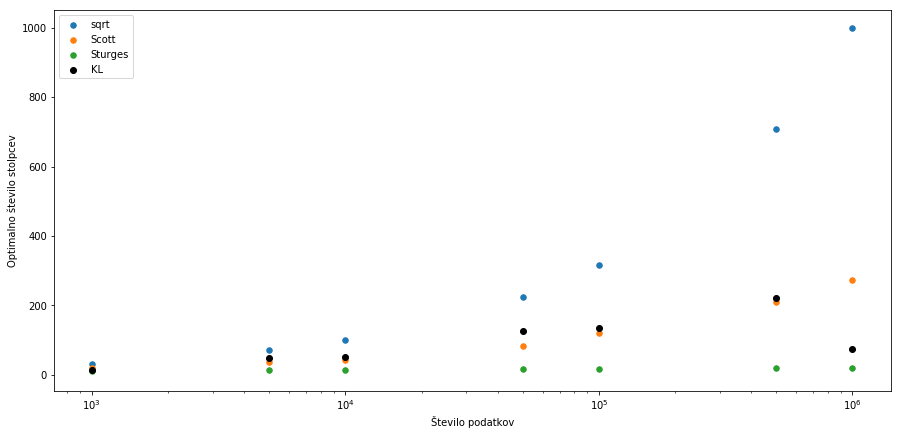
\includegraphics[width=\textwidth]{klVSostali}
    \caption{Primerjava med optimalnim številom stolpcev glede na korensko metodo in metodami Scott, Sturges in Kullback-Leibler. Os s številom podatkov je v logaritemski skali.}
\end{figure}

Zaradi preglednosti smo metodi Freedman-Diaconis in Rice izpustili. Iz slike je razvidno, da Kullback-Leibler metoda daje optimalna števila stolpcev podobna tistim, ki jih dajo ostale metode. Je pa izračun optimalnega števila stolpcev po Kullback-Leibler metodi zelo počasen, ko je število podatkov veliko. Prav tako pa procesa ne moremo optimizirati, saj funkcija $f(n) = D_{KL}(p\|h_n)$ ni konveksna, kar bi nam omogočilo iskanje minimuma, torej moramo direktno $m$-krat izračunati vrednost Kullback-Leibler divergence, kar pa je zaradi integriranja časovno zamudno.


\section{Renyi divergenca glede na histogram}\label{posplositev1d}

Zdaj, ko dobro poznamo pojem histograma, lahko definiramo Renyi divergenco glede na histogram. Histogram bo torej ocena za gostoto verjetnosti vzorca.

V prejšnjem poglavju smo omenili, da lahko histogram predstavimo kot funkcijo, a bo za računanje Renyi divergence boljše, da si histogram predstavljamo grafično. Torej predstavljamo si ga kot skupek pravokotnikov (stolpcev) z določenimi mejami in višinami.

\subsection{Formula za računanje Renyi divergence glede na histogram}

\begin{izrek}
    Naj bo $H_1$ histogram, ki ima meje stolpcev $(x_0,x_1,\ldots,x_{n-1}, x_n)$ in višine stolpcev $(h_{(1,0)},\ldots,h_{(1,n-1)})$. Naj bo $H_2$ histogram, ki ima meje stolpcev iste kot $H_1$ in višine stolpcev $(h_{(2,0)}, \ldots, h_{(2,n-1)})$ (torej imata $H_1$ in $H_2$ isto število stolpcev in enake meje, le različne višine). Tedaj lahko Renyi divergenco med histogramoma $H_1$ in $H_2$ izračunamo kot:
    \begin{equation}
        D_\alpha (H_1 \| H_2) = \frac{1}{\alpha-1} \log\Big(\sum_{i=0}^{n-1} h_{(1,i)}^\alpha \cdot h_{(2,i)}^{1-\alpha} \cdot (x_{i+1}-x_i)\Big),
    \end{equation}
    če $\alpha \neq 1$, oziroma
    \begin{equation}
        D_1 (H_1 \| H_2) = \sum_{i=0}^{n-1} h_{(1,i)}\cdot \log \frac{h_{(1,i)}}{h_{(2,i)}} \cdot (x_{i+1}-x_i).
    \end{equation}
\end{izrek}

\begin{proof}
    Vemo: če $H_1$ in $H_2$ zapišemo kot funkciji ($H_1 = H_1 (x)$ in $H_2 = H_2(x)$), dobljeni funkciji ustrezata pogojem za gostoto verjetnosti. Torej lahko izračunamo Renyi divergenco po definiciji:
    \begin{equation}
        D_{\alpha} (H_1 \| H_2) = \frac{1}{\alpha-1} \log\int_{x_0}^{x_n} H_1(x)^\alpha \cdot H_2(x)^{1-\alpha} dx.
    \end{equation}
    Ker sta funkciji $H_1$ in $H_2$ nezvezni v istih točkah (v mejah stolpcev), zapišemo integral kot vsoto integralov na intervalih, kjer sta $H_1$ in $H_2$ konstantni:
    \begin{equation}
        \int_{x_0}^{x_n} H_1(x)^\alpha \cdot H_2(x)^{1-\alpha} dx = \int_{x_0}^{x_1} H_1(x)^\alpha \cdot H_2(x)^{1-\alpha} dx + \ldots + \int_{x_{n-1}}^{x_n} H_1(x)^\alpha \cdot H_2(x)^{1-\alpha} dx.
    \end{equation}
    Če upoštevamo še konstantne vrednosti funkcij $H_1$ in $H_2$ na intervalih integriranja, in v vsakem členu integriramo $\int_a^b dx = b-a$, dobimo:
    \begin{equation}
        h_{(1,0)}^\alpha\cdot h_{(2,0)}^{1-\alpha}\cdot (x_1-x_0) + \ldots + h_{(1,n-1)}^\alpha\cdot h_{(2,n-1)}^{1-\alpha}\cdot (x_n-x_{n-1}) = \sum_{i=0}^{n-1} h_{(1,i)}^\alpha \cdot h_{(2,i)}^{1-\alpha} \cdot (x_{i+1}-x_i),
    \end{equation}
    torej je:
    \begin{equation}
        D_\alpha (H_1 \| H_2) = \frac{1}{\alpha-1} \log\Big(\sum_{i=0}^{n-1} h_{(1,i)}^\alpha \cdot h_{(2,i)}^{1-\alpha} \cdot (x_{i+1}-x_i)\Big).
    \end{equation}
    Podobno dokažemo za $\alpha = 1$ - izračunamo Kullback-Leibler divergenco.
\end{proof}

Zdaj znamo izračunati Renyi divergenco med dvema histogramoma, a imamo zelo strogo omejitev: meje stolpcev prvega histograma morajo biti enake mejam stolpcev drugega histograma. Opišimo, kako v splošnem primeru zadostimo tej omejitvi, brez da spreminjamo ploščine histogramov.

% rezanje histogramov
\subsection{Sprostitev definicijskega območja histogramov} \label{podpoglavje-4-1}

Če hočemo, da imata poljubna histograma enake meje stolpcev, moramo najprej uskladiti definicijski območji histogramov.

Naj bo $X$ urejen seznam z mejami stolpcev prvega histograma in $Y$ urejen seznam z mejami stolpcev drugega histograma. Za spodnjo mejo:
\begin{itemize}
	\item Če je $\min(X) > \min(Y)$, potem na začetek seznama $X$ vstavimo element $\min(Y)$. Tako v prvem histogramu dobimo še en stolpec z mejami $\min(Y)$ in $\min(X)$. Dodelimo mu vrednost $0$.
	\item Če je $\min(X) < \min(Y)$, potem na začetek seznama $Y$ vstavimo element $\min(X)$. Tako v drugemu histogramu dobimo še en stolpec z mejami $\min(Y)$ in $\min(X)$. Dodelimo mu vrednost $0$.
\end{itemize}
Za zgornjo mejo:
\begin{itemize}
	\item Če je $\max(X) < \max(Y)$, potem na konec seznama $X$ vstavimo element $\max(Y)$. Tako v prvem histogramu dobimo še en stolpec z mejami $\max(X)$ in $\max(Y)$. Dodelimo mu vrednost $0$.
	\item Če je $\max(X) > \max(Y)$, potem na konec seznama $Y$ vstavimo element $\max(X)$. Tako v drugem histogramu dobimo še en stolpec z mejami $\max(Y)$ in $\max(X)$. Dodelimo mu vrednost $0$.
\end{itemize}
Dobili smo torej največ dva nova stolpca. Ker smo jima dodelili vrednost $0$, ploščina histograma ostaja enaka, torej je bil to dober korak k našemu cilju (da bodo ploščine histogramov čim bližje 1). Definicijsko območje obeh histogramov je na sedaj enako.

\begin{zgled}

Poglejmo si primer, kako sprostimo definicijsko območje histograma.

\begin{figure}[!bh]
    \centering
    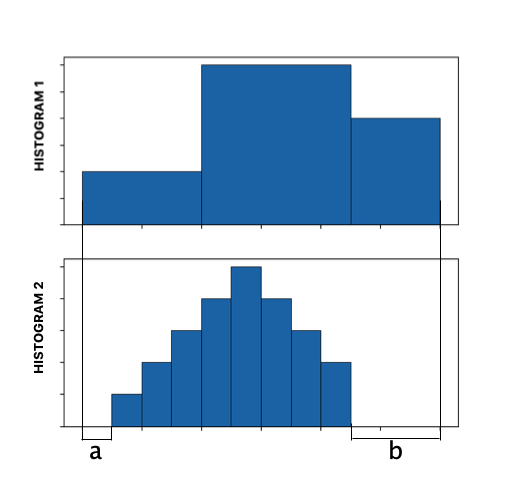
\includegraphics[scale=0.7]{definicijskoobmocje}
    \caption{Sprostitev definicijskega območjahistograma 2. Dobili smo dva nova stolpca ain b.}
\end{figure}

\end{zgled}
\pagebreak
\subsection{Prerazporeditev mej v histogramih}
Ko imamo histograma, definirana na enakem definicijskem območju, moramo uskladiti še meje stolpcev obeh histogramov. To naredimo tako, da združimo meje prvega in drugega histograma.

Naj bo $X$ urejen seznam z mejami prvega histograma in $Y$ urejen seznam z mejami drugega histograma. Tvorimo seznam $Z = X \cup Y$ in ga uredimo po velikosti od najmanjšega do največjega. Dolžina seznama $Z$ naj bo enaka $n$. Cilj je, da imata na koncu naša histograma razporeditev stolpcev ravno $Z$. Zdaj že vemo, da imata $X$ in $Y$ enak prvi in zadnji element (zaradi sprostitve definicijskega območja). Naj predstavlja zapis $A(i)$ i-ti element seznama $A$, vsak seznam pa vedno začnemo šteti z 1.

Ker že vemo, da bo na koncu veljala enakost $X = Z$, se osredotočimo le na vrednosti oz. višin stolpcev v prvem histogramu z novimi mejami.

Brez škode za splošnost lahko rečemo,  da je vrednost stolpca dodeljena prvi (manjši) meji stolpca. Tako ima vsak element $X(i)$ dodeljeno vrednost $X_v(i)$, ki predstavlja višino stolpca z mejami $X(i)$ in $X(i+1)$. Zadnji meji ni dodeljena nobena vrednost, brez škode za splošnost mu lahko priredimo vrednost 0.

Z zanko se sprehodimo čez seznam $Z$ (t.j. $i = 1, \cdots, n-1$, kjer je $n$ enak dolžini seznama $Z$) in ga primerjajmo s seznamom $X$. Vsakemu elementu $Z$ želimo dodeliti vrednost, tako da bo histogram z mejami $Z$ sovpadal s histogramom z mejami $X$. Prva elementa sta enaka, zato elementu $Z(1)$ dodelimo vrednost $X_v(1)$. Za vsak naslednji $i$ imamo dve možnosti:
\begin{itemize}
	\item Če je $Z(i) = X(i)$, elementu $Z(i)$ priredimo vrednost $X_v(i)$. 
	\item Če je $Z(i) \neq X(i)$, potem elementu $Z(i)$ priredimo enako vrednost, kot jo priredimo meji $Z(i-1)$, torej vrednost $X_v(i-1)$.
\end{itemize}
Za prvi histogram torej dobimo meje stolpcev $Z$ in višine stolpcev $Z_{v1}$, kjer je za $i = 1, \cdots, n-1$ elementu $Z(i)$ prirejena vrednost $Z_{v1}(i)$, zadnjemu elementu v seznamu $Z$ pa priredimo vrednost $0$.

Analogno primerjamo seznam $Z$ in $Y$. Tako za drugi histogram dobimo meje stolpcev $Z$ in višine stolpcev $Z_{v2}$, kjer je za $j = 1, \cdots, n-1$ elementu $Z(j)$ prirejena vrednost $Z_{v2}(j)$, zadnjemu elementu v seznamu $Z$ pa priredimo vrednost $0$.

Z zgornjim postopkom smo stolpce le "razbili" na več stolpcev z isto višino, tako da ploščina histograma ostaja enaka $1$.

\begin{zgled}
Na primeru iz podpoglavja \ref{podpoglavje-4-1} si poglejmo rezanje stolpcev.
\begin{figure}[h!]
	\centering
	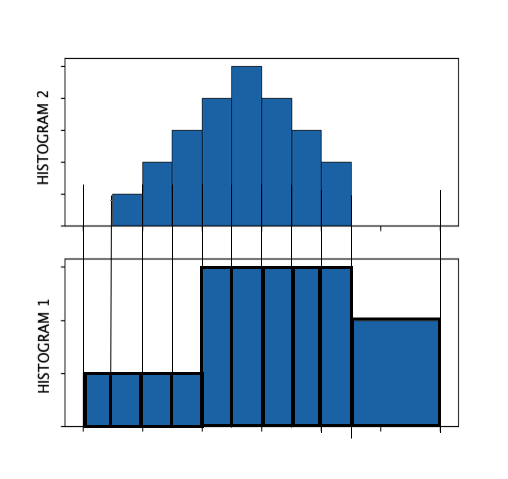
\includegraphics[scale=0.7]{prerazporeditev}
	\caption{Prerazporeditev mej stolpcev histograma 1 glede na histogram 2.}
    \end{figure}
    
\end{zgled}

Do sedaj smo med seboj primerjali le dve porazdelitvi. V nadaljevanju nas bo zanimal način, s katerim lahko primerjamo več porazdelitev hkrati. Za to pa moramo najprej vpeljati pojem entropije.

\section{Entropija}

Pojem entropije najdemo v fiziki in sociologiji, mi pa se bomo osredotočili na pomen tega pojma v statistiki.

Entropija je merilo za količino informacije, ki nam jo porazdelitev poda. Brez, da se poglabljamo v pojem entropije, navedimo defincijo Renyi entropije (glede na gostoto verjetnsti in glede na histogram).

\subsection{Renyi entropija glede na gostoto verjetnosti}

\begin{definicija}
    Naj bo $P$ porazdelitev z nosilcem $\Omega$, ki ji pripada gostota verjetnosti $p$. Naj bo $\alpha > 0$. \textbf{Renyi entropija glede na gostoto verjetnosti} je definirana kot:
    \begin{equation}
        H_{\alpha}(P)=\frac{1}{1-\alpha} \cdot \ln\int_{\Omega}\Big(p(x)\Big)^{\alpha}\  dx
    \end{equation}
    za $\alpha \neq 1$, za $\alpha = 1$ pa:
    \begin{equation}
        H(P)=-\int_{\Omega} p(x) \cdot \ln\Big(p(x)\Big) \  dx.
    \end{equation}
\end{definicija}

\begin{opomba}
    Renyi entropija za $\alpha = 1$ se imenuje Shannonova entropija. Dokaz, da je
    \begin{equation}
        \lim_{\alpha \rightarrow 1} H_\alpha(P) = H(P),
    \end{equation}
    je analogen dokazu, da je $\lim_{\alpha \rightarrow 1} D_\alpha (P \| Q) = D_{KL}(P \| Q)$, zato ga bomo izpustili. 
\end{opomba}

\pagebreak

\subsection{Renyi entropija glede na histogram}

\begin{izrek}
    Naj bo $H_1$ histogram, ki ima meje stolpcev $(x_0,x_1,\ldots,x_{n-1}, x_n)$ in višine stolpcev $(h_0,\ldots,h_{n-1})$. Naj bo $\alpha > 0$. Tedaj lahko Renyi entropijo histograma $K$ izračunamo kot:
    \begin{equation}
        H_\alpha(P) = \frac{1}{1-\alpha} \cdot \ln \  \Big( \sum_{1}^{n}(y_i^{\ \alpha} \cdot x_i) \Big),
        \end{equation}
    če $\alpha \neq 1$, oziroma za $\alpha = 1$:
    \begin{equation}
        H(P) = - \sum_{1}^{n}(y_i \cdot \ln y_i \cdot x_i).
    \end{equation}
\end{izrek}

\begin{opomba}
    Dokaz zgornjega izreka je analogen dokazu izreka za računanje Renyi divergence glede na histogram, zato ga izpustimo.
\end{opomba}

\subsection{Zgled}

Poglejmo si entropije za različne beta porazdelitve. Beta porazdelitev ima nosilec $[0,1]$ in je podana z dvema parametroma, recimo jima $a$ in $b$. Poglejmo, kako izgledajo gostote verjetnosti v odvisnosti od parametra.

\begin{figure}[!h]
    \centering
    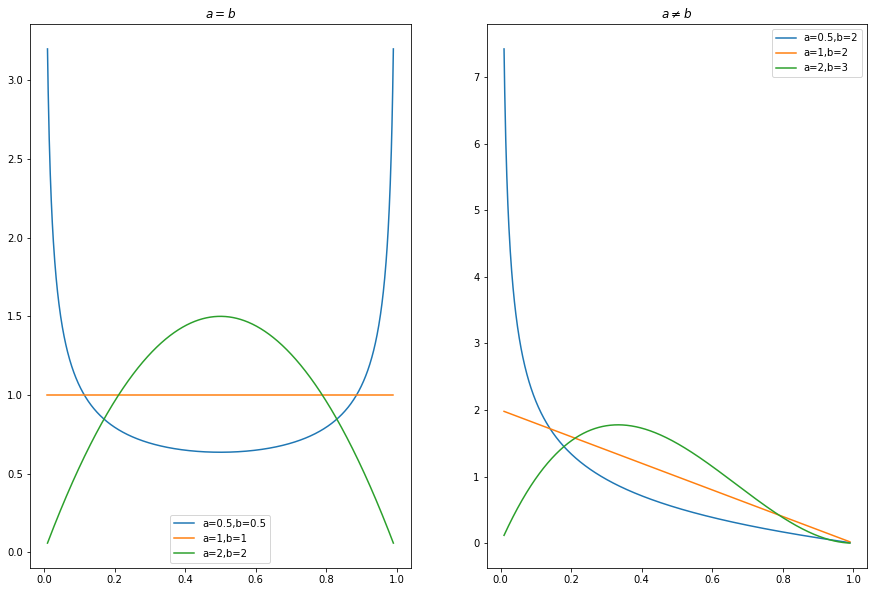
\includegraphics[width=0.7\textwidth]{bete.png}
    \caption{Gostote verjetnosti različnih beta porazdelitev.}
\end{figure}

Za te beta porazdelitve poglejmo graf Renyi entropij v odvisnosti od reda $\alpha$.

\begin{figure}[!h]
    \centering
    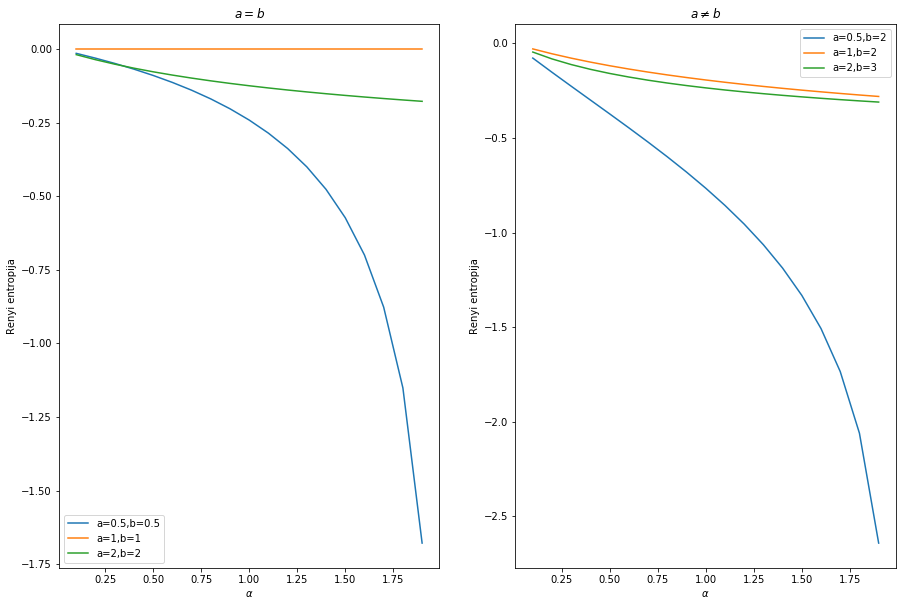
\includegraphics[width=\textwidth]{beteentropije.png}
    \caption{Entropije različnih beta porazdelitev.}
\end{figure}

Vidimo, da je entropija uniformne porazdelitve ($a = b = 1$) enaka 0 za vsak $\alpha$. Ta rezultat je pričakovan, saj nam uniformna porazdelitev ne pove nič, če poznamo nosilec porazdelitve (vemo, da bo naključen vzorec nekje na temu nosilcu.)

\section{Posplošena divergenca}

Posplošena divergenca je orodje, ki izračuna divergenco med več porazdelitvami hkrati, ne samo med dvema. Računali bomo torej lahko divergenco ansambla porazdelitev. Vpeljimo posplošeno Jensenovo divergenco.

\subsection{Razred Jensenovih divergenc}

Definirajmo razred Jensenovih divergenc.

\begin{definicija}
    Naj bo $H$ poljubna entropija. Naj bodo $P_1, \ldots, P_n$ porazdelitve na istem nosilcu in \\ $w = (w_1, \ldots, w_n)$ vektor uteži, tako da $\sum_{i=1}^n w_i = 1$. \textbf{Jensenova divergenca} je definirana kot:
    \begin{equation}
        J^w (P_1, \ldots, P_n) = H \Big(\sum_{i=1}^n w_i P_i\Big) - \sum_{i=1}^n w_i H(P_i).
    \end{equation}
\end{definicija}

Izpustimo dokaz, da ta razred res predstavlja razred divergenc. Vrstni red porazdelitev v Jensenovi divergenci je nepomemben, če so uteži enake ($\frac{1}{n}$). Nepomemben pa je tudi, če usklajeno permutiramo porazdelitve in uteži.

\subsection{Jensen-Renyi divergenca}

Ker smo v prejšnjem poglavju spoznali Renyi entropijo, si poglejmo Jensen-Renyi divergenco - torej Jensenovo divergenco, kjer za entropijo vzamemo Renyi entropijo.

\begin{definicija}
    Naj bo $H_\alpha$ Renyi entropija. Naj bodo $P_1, \ldots, P_n$ porazdelitve na istem nosilcu in \\ $w = (w_1, \ldots, w_n)$ vektor uteži, tako da $\sum_{i=1}^n w_i = 1$. Naj bo $\alpha > 0$. \textbf{Jensen-Renyi divergenca} je definirana kot:
    \begin{equation}\label{JRDformula}
        JR_\alpha^w (P_1, \ldots, P_n) = H_\alpha \Big(\sum_{i=1}^n w_i P_i\Big) - \sum_{i=1}^n w_i H_\alpha(P_i).
    \end{equation}
\end{definicija}

\subsection{Jensen-Renyi divergenca glede na histogram}

Zdaj, ko smo definirali Jensen-Renyi divergenco, nas zanima le-ta, ko so porazdelitve predstavljene s histogrami. Pojavi se namreč problem, saj moramo po definiciji Jensen-Renyi divergence v 1. členu formule \eqref{JRDformula} seštevati histograme med seboj.

Gostoto verjetnosti porazdelitve $P_i$ lahko predstavlja histogram z $m$ stolpci. Poimenujmo ta histogram kar $P_i$. Histogram $P_i$ lahko zapišemo kot $K_i = (x_i, y_i)$, kjer so $x_i = (x_{i,1}, \ldots, x_{i, m+1})$ meje stolpcev histograma $P_i$, $y_i = (y_{i,1}, \ldots, y_{i,m})$ pa višine stolpcev histograma $P_i$, kjer je $m$ enak številu stolpcev histograma $P_i$.

Da lahko izračunamo 1. člen v formuli \eqref{JRDformula}, moramo histograme pretvoriti na histograme z enakim definicijskim območjem in enakimi mejami stolpcev. To naredimo iterativno s postopki iz poglavja \ref{posplositev1d}. Ne rabimo pa spreminjati stolpcev z višino 0, saj pri računanju Renyi entropije ne pride do deljenja z 0. $\sum_{i=1}^n w_i P_i$ bo, ko jo izračunamo, ravno histogram, kjer seštejemo višine stolpcev, pomnožene z utežjo. Če zapišemo $P_i$ kot zgoraj, dobimo višine tega histograma:
\begin{align}
	\sum_{i=1}^n w_i P_i &= \sum_{i=1}^n w_i \cdot (x, y_i) \overset{(\ast)}{=} \\
	&\overset{(\ast)}{=} \Big(x_i, \sum_{i=1}^n w_i \cdot y_i\Big) = P^\prime,
\end{align}
kjer smo pri $\overset{(\ast)}{=}$ upoštevali, da spreminjamo le višine stolpcev in ne njihovih mej. Ker imajo po ureditvi definicijskega območja in mej stolpcev vsi histogrami iste meje, smo te meje poimenovali kot $x$.

V drugem členu nimamo težav, saj že znamo izračunati Renyi entropijo glede na histogram. Splošna formula za računanje Jensen-Renyi divergence glede na histogram se torej glasi:
\begin{equation}
    JR_\alpha^w (P_1, \ldots, P_n) = H_\alpha (P^\prime) - \sum_{i=1}^n w_i H_\alpha(P_i).
\end{equation}

\pagebreak

\subsection{Uporaba Jensen-Renyi divergence}

Opišimo primer uporabe Jensen-Renyi divergence. Recimo, da želimo sporočiti napako na stroju, ko se ta pojavi. Imamo histograme oz. gostote verjetnosti, ki predstavljajo optimalno delovanje stroja (predstavljajo lahko npr. temperaturo, vibracije, glasnost, \ldots).

Vzamemo polurni interval, ko bomo preverjali delovanje stroja. Torej v pol ure bomo zbrali dovolj podatkov, da bomo lahko skonstruirali histograme ali gostote verjetnosti, ki bodo predstavljali trenutno delovanje stroja.

Izračunajmo Jensen-Renyi divergenco ansambla histogramov, ki predstavljajo optimalno delovanje stroja - recimo, da dobimo vrednost $x$. Sedaj pa izračunajmo še Jensen-Renyi divergenco trenutnega delovanja - recimo, da dobimo vrednost $y$. Razlika $|x-y|$ lahko meri, kolikšno je odstopanje trenutnega delovanja od optimalnega. Lahko si postavimo mejo $c$, ko bomo sporočili napako. Napako bomo torej sporočili, če bo $|x-y| > c$.


\section{Zaključek}

Spoznali smo nekaj metod, ki jih lahko uporabimo v realnih problemih odkrivanja napak delovanja. Predvsem je pomembno, da imamo na voljo dovolj podatkov, da lahko zgradimo verodostojen histogram ali gostoto verjetnosti. Če imamo premalo podatkov, je lahko prirejen histogram daleč od realnega. Seveda pa je zbiranje zadostnega števila podatkov finančno pogojeno.

Ugotoviti moramo tudi, kakšne časovne intervale bomo izbrali za preverjanje delovanja. Če izberemo le eno dolžino intervala, se lahko napaka razporedi na dva intervala in je ne bomo zaznali. To lahko rešimo tako, da vzporedno preverjamo pravilnost z istim intervalom, ki pa bo v vzporedni liniji za polovico zamaknjen.

Jasno pa je, da obstaja neka praktična zgornja meja za število podatkov, ki jih lahko zajamemo. To pomeni, da bo cena senzorja za merjenje naraščala eksponentno v odvisnosti od frekvence zajema podatkov. Narediti moramo torej kompromis med ceno, ki smo jo pripravljeni plačati, in kvaliteto merjenja napake.

\newpage

%---------------------------------------------------
% VIRI
%---------------------------------------------------
\bibliographystyle{plain}
% \bibliography{sample.bib}

\begin{thebibliography}{9}
	
\bibitem{knjiga}
Dekking, F. M., Kraaikamp, C., Lopuha{\"a}, H. P. in Meester, L. E., 2005. A Modern Introduction to Probability and Statistic: Understanding Why and How. 2. izdaja. London: Springer-Verlag London Limited.

\bibitem{eguchi}
Eguchi, S., 1985. A differential geometric approach to statistical inference on the basis of contrast functional. Dostopno na: \url{https://projecteuclid.org/download/pdf_1/euclid.hmj/1206130775} [9. 3. 2019]

\bibitem{fdv}
Ferligoj, Anu\v{s}ka, idr. 2015, Osnove statistike na prosojnicah: \v{s}tudijsko gradivo pri predmetu Statistika, Ljubljana: Fakulteta za dru\v{z}bene vede.

\bibitem{Gil}
Gil, M., 2011. On Rényi Divergence Measures for Continuous Alphabet Sources. Dostopno na: 
\url{https://pdfs.semanticscholar.org/8ebc/dd48e51d9f18a0025794ae088ce754dd47ce.pdf} [9. 3. 2019]

\bibitem{bf}
Košmelj, K., 2007. Uporabna statistika. 2. izdaja. Ljubljana: Biotehniška fakulteta.

\bibitem{sason}
Sason, I. in Verd\'u, S., 2018. f-Divergence Inequalities. Dostopno na: \url{http://webee.technion.ac.il/people/sason/f-divergence%20inequalities.pdf} [9. 3. 2019]

\bibitem{vanErven} 
van Erven, T. in Harremoës, P., 2007. Renyi Divergence and Kullback-Leibler Divergence. Dostopno na: 
\url{https://arxiv.org/pdf/1206.2459.pdf} [9. 3. 2019]

\end{thebibliography}

\end{document}